\documentclass[10pt,letterpaper,twoside]{report}
%\usepackage{manuscript}
\usepackage{amsmath}
\usepackage{amsfonts}
\usepackage{amssymb}
\usepackage{graphicx}
\usepackage{tabularx}
\usepackage{algorithm}
\usepackage{algpseudocode} 
\usepackage{url}
\usepackage[english]{babel}



%\usepackage{venturis2}

\linespread{1.0}
\title{Proposal}
\author{Andrew Rosen}
\begin{document}



\maketitle
\setcounter{tocdepth}{4}
\tableofcontents
\newpage

\begin{abstract}
Distributed Hash Tables (DHTs) are protocols and frameworks used by peer-to-peer (P2P) systems.
They are used as the organizational backbone for many P2P file-sharing systems due to their scalability, fault-tolerance, and load-balancing properties.
These same properties are highly desirable in a distributed computing environment, especially one that wants to use heterogeneous components.
DHTs can be used not only as the framework to build a P2P file-sharing service, but a P2P distributed computing platform.

Our framework is a completely decentralized framework for organizing heterogeneous units for distributed computation.
It incorporates a load-balancing algorithm that is capable of injecting additional nodes during runtime to speed up existing jobs.
This algorithm also provides a means of redistributed the load among existing workers during runtime.

%applications
Unlike Hadoop and similar MapReduce frameworks, our framework can be used both in both the context of a datacenter or as part of a P2P computing platform.  
This opens up new possibilities for building platforms to distributed computing problems.
By utilizing the load-balancing algorithm, a datacenter could easily leverage additional P2P resources at runtime on an as-needed basis.
Our framework also allows MapReduce-like or distributed machine learning platforms to be easily deployed in a greater variety of contexts.

\end{abstract}

%TODO: Replace first person singulars with first person plurals
%TODO: Split proposal into Finished research and proposed experiments.
%TODO: Rewrite vocab
%TODO: Add pretty pictures for DHT
%TODO: Add motivation of Sybil attacks on Botnets
\chapter{Introduction}
\label{chapter:intro}
% % % layout
% % % Distributed Computing Challenges
% % % Qualities of DHTs
% % % Hypothesis = These Problems + These qualiteies -> solution
% % % Framework of what these solutions are and what they can do


%TODO: Create intro paragraph with paragraph from abstract
%TODO: Get some structure!  Move background to background, this section should be purely motivation;  tell what dht's can do right now and what proposed uses there are and what YOU propose.  Also incorperate the challenges you need to overcome.  You can say these things are hard for DHTs and we'll tell you more in background.
%TODO:  Make sure you have roadmap:  Highlevel What you have done, what you plan to do.

Distributed Hash Tables (DHTs) are protocols and frameworks used by peer-to-peer (P2P) systems.
They are used as the organizational backbone for many P2P file-sharing systems due to their scalability, fault-tolerance, and load-balancing properties.
These same properties are highly desirable in a distributed computing environment, especially one that wants to use heterogeneous components.
DHTs can be used not only as the framework to build a P2P file-sharing service, but a P2P distributed computing platform.


% What do I want to do?
\section{Objective}
Our goal is to create a framework to further generalize Distributed Hash Tables (DHTs) to be used for distributed computing.
Distributed computing platforms need to be scalable, fault-tolerant, and load-balancing.
%The ability to incorporate heterogeneous hardware is a definite benefit.
We will discuss what each of these mean and why they are important in section \ref{sec:challenges}, but briefly:

\begin{itemize}
	\item The system should be able to work effectively no matter how large it gets.
	As the system grows in size, we can expect the overhead to grow in size as well, but at an extremely slower rate.
	\item The more machine integrated into the system, the more we can expect to see hardware failures.
	The system needs to be able to automatically handle these hardware failures.
	\item Having a large number of machines to use is worthless if the amount of work is divided unevenly among the system.
	The same is true if the system hands out larger jobs to less powerful machines or smaller jobs to the more powerful machines.
	%\item We cannot assume that we be able to replace our broken machines with exact replicas, nor do we assume we would want to. 
\end{itemize}


These are many of the same challenges that Peer-to-peer (P2P) file sharing applications have.
Many P2P applications use DHTs to address these challenges, since DHTs are designed with these problems in mind.
We propose that DHTs can be used to create P2P distributed computing platforms that are completely decentralized.
%Rather than keys being assigned to some data, we can assign keys to tasks and automatically distribute those tasks to the responsible nodes
There would be no need for some central organized or scheduler to coordinate the nodes in the network.
Our framework would not be limited to only a P2P context, but could be applied in data centers, a normally centrally organized context.


A successful DHT-based computing platform would need to address the problem of dynamic load-balancing.
This is currently an unsolved\footnote{As far as we know.} problem. %I have to check a couple of papers of to confirm.
If an application can dynamically reassign work to nodes added at runtime, this opens up new options for resource management.
Similarly. if a distributed computation  is running too slow, new nodes can be added to the network during runtime or idle nodes can boot up more virtual nodes. %(now that I think of it this is two different but highly related problems: internal and external).

%Move this bit to the end?
Chapter \ref{chapter:background} will delve into how DHTs work and examine specific DHTs.
The remainder of the proposal will then discuss the work we plan on doing to demonstrate the viability of using DHTs for distributed computing.



% How I will do it is in the experiments chapter

% Why should you care?
\section{Applications of Distributed Hash Tables}

Distributed Hash Tables have been used in numerous applications:

\begin{itemize}
	\item \textit{P2P file sharing} is by far the most prominent use of DHTs.  
	The most well-known application is BitTorrent \cite{bittorrent}, which is built on Mainline DHT \cite{mainline}.
	\item DHTs have been used for \textit{distributed storage} systems \cite{CFS}.
	\item \textit{Distributed Domain Name Systems} (DNS) have been built upon DHTs \cite{cox2002serving} \cite{pappas2006comparative}.
	Distributed DNSs are much more robust that DNS to orchestrated attacks, but otherwise require more overhead.
	%\item Distributed search (faroo)
	\item DHT was used as the name resolution layer of a large \textit{distributed database} \cite{Mateescu2011440}.
	\item Distributed \textit{machine learning} \cite{liparameter}.
	\item Many \textit{botnets} are now P2P based and built using well established DHTs \cite{saad2011detecting}. 
	This is because the decentralized nature of P2P systems means there's no single vulnerable location in the botnet.
	\item \textit{Live video streaming} (BitTorrent live) \cite{mol2009design}.
\end{itemize}

We can see from this list that DHTs are primarily used in P2P applications, but other applications, such as botnets, use DHTs for their decentralization.
We want to use DHTs primarily for their intuitive\footnote{Relatively intuitive, if you know how hash tables work.} way of organizing a distributed system.

We showed  \cite{chordreduce} that a DHT can be to create a distributed computing framework.
We used the same mechanism used in P2P applications that assigns nodes their location in the network to evenly distribute work among members of a DHT.
The most direct application of a DHT distributed computing framework is  a quick and intuitive way to solve embarrassingly parallel problems, such as:
\begin{itemize}
	\item Brute force cryptography.
	\item Genetic algorithms.
	\item Markov chain Monte Carlo methods.
	\item Random forests.
	\item Any problem that could be phrased as a MapReduce problem.
	
\end{itemize}
Unlike the current distributed applications which utilize DHTs, we want to create a complete framework which can be used to build decentralized applications.
We have found no existing projects that provide a means of building your own DHT or DHT based applications. %without a given DHT in mind at least


% So you're diong these things with this tool
\section{Why Use Distributed Hash Tables in Distributed Computing}
% Okay so this is all great, but what's special about a DHT
% First, let's talk about the problems with distributed computing

Using distributed hash tables for distributed computing is not necessarily the most intuitive step.
To understand why we want to use DHTs for distributed computing, we will first examine some of the more prominent challenges in distributed computing.

\subsection{General Challenges of Distributed Computing}
\label{sec:challenges}

As we mentioned earlier, distributed computing platforms need to be scalable, fault-tolerant, and load-balancing.
We will look at these individually:


\begin{description}
	\item[Scalability] - Distributed computing platforms should not be completely static and should grow to accommodate new needs.
	However, as systems grow in size, the cost of keeping that system organized grows too.
	The challenge of scalability is designing a protocol that grows this organizational cost at an extremely slow rate.
	For example, a single node keeping track of all members of the system might be a tenable situation up to a certain point, but eventually, the cost becomes too high for a single node.
	%not sure about this line
	We want this organizational cost spread among many nodes to the point where this cost is insignificant. % 
	\item[Fault Tolerance]  
	The quality of fault-tolerance or \textit{robustness} \footnote{There is apparently a subtle difference between fault-tolerance and robustness, but we will use the two interchangeably here until we get told to stop.} means that the system still works even after a component breaks (or many components break).
	We want our platform to gracefully handle failures during runtime and be able to quickly reassign work to other workers.
	In addition, the network should be equally graceful in handling the introduction of new nodes during runtime.
	
	\item[Load-Balancing]
	The challenge of load balancing is to evenly distribute the work among nodes in the network.
	This is always an approximation; rarely  are there exactly enough pieces for  every node to get the same amount of work.
	The system needs an efficient set of rules for dividing arbitrary jobs into small pieces and sending those pieces to the nodes.
	
	A subproblem here is handling \textit{heterogeneity},\footnote{It could even be considered a problem in its own right.} or how should the system should handle different pieces of hardware with different amounts of computational power.
	
	
\end{description}
It should be noted that there is some crossover between these categories. 
For example, adding new nodes to the system needs to have a low organizational overhead (scalability) and will change the network configuration, which will need to be updated (fault-tolerance).


%move below
%One question we are particularly interested in answering touches on all three categories:  can we do load balancing during run-time?
%A goal we have is t


\subsection{How DHTs Address these Challenges}
%Without getting into the details of what a DHT is, what do they do?
Distributed Hash Tables are essentially distributed lookup tables.
DHTs use a consistent hashing algorithm, such as SHA-1 \cite{sha1}, to associate nodes and file identifiers with keys.  
These keys dictate where the nodes and files will be located on the network.
The connections between nodes are organized such that any node can efficiently lookup the value associated with any given key, even though the node only knows a small portion of the network.
We discuss the specifics this in Chapter \ref{chapter:background}.

Nearly every DHT was designed with large, P2P applications in mind, with millions of nodes in the network and new nodes entering and leaving all the time.
This has lead to DHTs being designed with specific qualities in mind.

\paragraph{Scalability}
The organization responsibility in DHTs is spread among all members of the network.
Each node only knows a small subset of the network,\footnote{Except for ZHT \cite{li2013zht}, which breaks this rule deliberately and with gusto by giving each node a full copy of the routing table.} but can use the nodes it knows to efficiently find any other node in the network.
Because each individual node only knows a small part of the network, the maintenance costs associated with organization are correspondingly small.

Using consistent hashing allows the network to scale up incrementally, adding one node at a time \cite{dynamo}.
In addition, each join operation has minimal impact on the network, since a node affects only its immediate neighbors on a join operation.
Similarly, the only nodes that need to react to a node leaving are its neighbors.
Other nodes can be notified of the missing node passively through maintenance or in response to a lookup.

There have been multiple proposed strategies for tackling scalability, and it is these strategies which play the greatest role in driving the variety of DHT architectures. 
Each DHT must strikes a balance between size of the lookup table and lookup time. 
The vast majority of DHTs choose to use $\lg(n)$ sized tables and  $\lg(n)$ hops. 
Chapter \ref{chapter:background} discusses these tradeoffs in greater detail and how they affect the each DHT.


\paragraph{Fault-Tolerance}
One of the most important assumptions of DHTs is that they are deployed on a constantly changing network.
DHTs are built to account for a high level of \textit{churn}.\footnote{Again, except for ZHT.}  
\textit{Churn} is the disruption of routing caused by the constant joining and leaving of nodes.
In other words, the network topology is assumed to always be in flux.
This is mitigated by a few factors.

First, the network is decentralized, with no single node acting as a single point of failure.
This is accomplished by each node in the routing table having a small portion of the both the routing table and the data stored on the DHT.

Second is that each DHT has an inexpensive maintenance processes that mitigates the damage caused by churn.
DHTs often integrate a backup process into their protocols so that when a node goes down, one of the neighboring nodes can immediately assume responsibility.
The join process also slightly disrupt the topology, as affected nodes must adjust their peerlists to accommodate the joiner. 

The last property is that the hashing algorithm used to distribute content evenly across the DHT also distributes nodes evenly across the DHT.  
This means that nodes in the same geographic region occupy vastly different locations in the network.  
If an entire geographic region is affected by a network outage, this damage is spread evenly across the DHT, which can be handled, rather than a contiguous portion.

%This property is the most important, as it deals with failure of entire sections of the network, rather than a single node.
%Recent research in using DHTs for High End Computing \cite{li2013zht} shows what can happen if we remove this assumption by working with an almost completely static network.

The fault tolerance mechanisms in DHTs also provide near constant availability for P2P applications.
The node that is responsible for a particular key can always be found, even when numerous failures or joins occur \cite{chord}.


\paragraph{Load-Balancing}
Consistent hashing is also used to ensure load-balancing in DHTs.
Consistent hashing algorithms associate nodes and file identifiers with keys.  
These keys are generated by passing the identifiers into a hash function, typically SHA-160.
The chosen hash function is typically large enough to avoid hash collisions\footnote{A hash collision occurs when the hashing algorithm outputs the same hashkey for two different inputs.} and generates keys in a uniform manner. 

Essentially, both nodes and data are spread about the network uniformly at random.
Nodes are responsible for the files with keys ``close'' to their own.
What ``close'' means depends on the specific implementation. 
we found defining the meaning of ``close'' equivalent choosing a metric for Voronoi tessellation \cite{vhash}.
However, because this is a random process, not all values are evenly distributed, but enough hash keys yield a close enough approximation.

Heterogenity presents a challenge for load-balancing DHTs due to conflicting assumptions and goals. 
DHTs assume that members are usually going to be varied in hardware, but the load-balancing process defined in DHTs treats each node equally.s
In other words, DHTs support heterogeneity, but do not attempt to exploit it.

This doesn't mean that heterogeneity cannot be exploited.
Nodes can be given addition responsibilities manually, by running multiple instances of the P2P application on the same machine or creating more virtual nodes.
%TODO:  Heat dissipation citation.

%However, this is not a feasible option for any kind of truly decentralized system and would need to be done automatically.
%There is no well-known mechanism to that exists to automatically allocate virtual nodes on the fly \footnote{citation needed, although this can be similar to IRM}. 


\section{Roadmap}

In this section, we give a brief overview of our previous work.
We go into further detail of our previous work in Chapter \ref{chapter:prev} and we enumerate the pieces of our dissertation in Chapter \ref{chapter:experiments}. 
\subsection{Completed Work}

%chord reduce
One of our first projects was to create a distributed computing platform using the Chord DHT \cite{chordreduce}.
Our goal here was to create a completely decentralized distributed computing framework which was fault-tolerant during job execution.
We did this by implementing MapReduce over Chord.
We then tested our prototype's fault-tolerance by executing MapReduce jobs under churn.

Our experiments with ludicrously high levels of churn created an anomaly in the runtime of our computations.
Under absurd levels of experimental churn, we found that our computation was quicker than our experiments without churn.
We hypothesize that this is because the random churn is acting as a (inefficient) process for autonomous load-balancing.
This phenomena is described in detail in Chapter \ref{sec:auto-load-bal}, but suggested to us that there was a way to  dynamically load-balance during execution.

%VHash as the ur-example
The second project we worked on was VHash \cite{vhash} \cite{dgvh}, a distributed hash table based on Delaunay Triangulation.
VHash is unique for the way it could work in multidimensional spaces.

We discovered the closeness metric used by DHTs to determine which node is responsible for what data is analogous to the metric used to create a Voronoi tessellation.
This means the neighbors of the node map to Delaunay triangulations. 
To the best of our knowledge, no other party has inferred the relationship between Voronoi tessellations, Delaunay triangulations and distributed hash tables.
These properties gives us a way to postulate an \textit{ur}-DHT, a progenitor DHT which could be used to define all other DHTs.


%DGVH shows that DHTs function even when the closeness metric is fuzzy


%Sybil
We also did a project which analyzed the amount of effort that would be required to attack a DHT using a method known as the Sybil attack \cite{sybil-analysis}.
The Sybil attack \cite{sybil} is a well known attack against distributed systems, but it had not been fully analyzed from the perspective of an attacker.
We believe that some of the components that are used to perform a Sybil attack can be used for autonomous load balancing.

%looking for publication


%distributed DNS:  experience building DHTs
\subsubsection{Published Work}

\begin{itemize}
	\item Andrew Rosen, Brendan Benshoof, Robert W. Harrison, Anu G. Bourgeois ``MapReduce on a Chord Distributed Hash Table'' Presentation ICA CON 2014, Poster at IPDPS 2014 PhD Forum \cite{chordreduce}
	\item Brendan Benshoof, Andrew Rosen, Anu G. Bourgeois, Robert W. Harrison ``VHASH: Spatial DHT based on Voronoi Tessellation'' Poster and Short Paper ICA CON 2014 \cite{vhash}
	\item Brendan Benshoof, Andrew Rosen, Anu G. Bourgeois, Robert W. Harrison ``A Distributed Greedy Heuristic for Computing Voronoi Tessellations With Applications Towards Peer-to-Peer Networks'' IEEE IPDPS 2015 - Workshop on Dependable Parallel, Distributed and Network-Centric Systems \cite{dgvh}
	
\end{itemize}




	

I also have a number of publications with other authors not relevant to the proposed work.
\begin{itemize}
	\item  Erin-Elizabeth A. Durham, Andrew Rosen, Robert W. Harrison
	``A Model Architecture for Big Data applications using Relational Databases''
	2014 IEEE BigData - C4BD2014 - Workshop on Complexity for Big Data  \cite{durham2014model}
	\item Chinua Umoja, J.T. Torrance, Erin-Elizabeth A. Durham, Andrew Rosen, Dr. Robert Harrison
	``A Novel Approach to Determine Docking Locations Using Fuzzy Logic and Shape Determination''
	2014 IEEE BigData - Poster and Short Paper \cite{umoja2014novel}
	\item  Erin-Elizabeth A. Durham, Andrew Rosen, Robert W. Harrison
	``Optimization of Relational Database Usage Involving Big Data'' 
	IEEE SSCI 2014 - CIDM 2014 - The IEEE Symposium Series on Computational Intelligence and Data Mining \cite{durham2014optimization}
\end{itemize}

\subsection{Summary of Proposal}


The work we want to do can be divided into three distinct, but mutually dependent parts.
One of these parts, the DHT framework, is a part that will be done jointly with Brendan Benshoof.
The specifics are given in Chapter \ref{chapter:experiments}.


\subsubsection{DHT Framework}
The goal of the DHT framework is to create a ready-to-use framework for creating DHT applications.
We will then use this to create the DHT applications for the DHT distributed computing.
This section should produce one to two publications:  one for the framework itself and how our abstractions can be used to create any DHT, the other will be on expanding our VHash publication \cite{vhash}.

The framework will be developed in either Go or Python3.
These two languages are being considered due to their ease of programming.

%significance is abstractions and our Voronoi definitations 

\subsubsection{DHT Distributed Computing}

This portion will be the bulk of the experimental work and data gathering.
Using our created framework, we will create implement and test distributed computing problems on different DHT implementations, such as Chord \cite{chord} and Kademlia \cite{kademlia}.

\subsubsection{Autonomous Load-Balancing}
Our goal here is to develop a new and efficient algorithm for balancing the workload among members of the DHT.
Load balancing schemes do exist for file storage, but none exist for computation.
Furthermore, we want to develop a system that takes into account the heterogeneity of a given system, allowing more powerful nodes to take on more responsibility.



%\section{Old stuff starts here}



%Distributed Hash Tables (DHTs) are traditionally used as the backbone of structured Peer-to-Peer (P2P) file-sharing applications.
%The largest such application is Bittorrent \cite{bittorrent}, which is built using Mainline DHT \cite{mainline},  a  derivative of Kademlia \cite{kademlia}.
%The number of users on Bittorrent ranges from 15 million to 27 million users daily, with a turnover of 10 million users a day \cite{mainlineMeasure}.

%Most research on DHTs assumes that DHTs will be used in the context of a large P2P file-sharing application (or at least, an application \textit{potentially} incorporating millions of nodes).
%This leads the DHT to having particular qualities.
%The application must be scalable and no single node knows every other node in the network.
%The network must be able to handle members joining and leaving arbitrarily.
%The resulting application must be agnostic towards hardware.
%The network must be decentralized and split whatever burden there is equally among its members.

%In other words, distributed hash tables provide scalability, fault-tolerance, and load-balancing to an application.
%Recent applications have leveraged these qualities, since these qualities are desirable in many different frameworks.
%For example, one paper \cite{Mateescu2011440} used a DHT as the name resolution layer of a large distributed database.
%Research has also been done in using DHTs as an organizing mechanism in distributed machine learning \cite{liparameter}. 

 %e describe each of the aforementioned qualities and their ramifications below in sections \ref{subsec:ft}, \ref{subsec:lb}, \ref{subsec:scalability}, and \ref{subsec:hetero} .
% While these properties are individually enumerated, they are greatly intertwined and the division between their impacts can be somewhat arbitrary.

%\subsubsection{Load Balancing}
%\label{subsec:lb}



%This appears to be a weakness, but can be turned into an advantage in heterogeneous systems by using \textit{virtual nodes} \cite{dynamo} \cite{godfrey2005heterogeneity} .
%When a node joins the network, it joins not at one position, but multiple virtual positions in the network \cite{dynamo}.
%Using virtual nodes allows load-balance optimization in a heterogeneous network; more powerful machines can create more virtual nodes and handle more of the overall responsibility in the network.
%Load balancing is still an active area of research for DHTs.


%DeCandia et al\. discussed various load balancing techniques that were tested on Dynamo \cite{dynamo}.  
%Each node was assigned a certain number of tokens and the node would create a virtual node for each token.
%The realization DeCandia et al\. had was that there was no reason to use the same scheme for data partitioning and data placement.
%DeCandia et al\. introduced two new strategies which work off assigning nodes equally sized partitions.


% HELP

%While most DHTs follow this scheme, there is some minor variation on how keys are generated.
%Some DHTs can or do use geographic information to generate keys.
%In VHash, keys are not static, but move according to a simplified spring model.

%\paragraph{Heterogeneity}
%\label{subsec:hetero}
%A few options present themselves.  % and are discuessed in \ref{}
%add the above if the below is moved

%This might be the wrong place for this
%One is to use adapt a request tracking mechanism, such as what is used in IRM, except instead of tracking file requests, it tracks requests that are directed to a particular (real) node. 
%If a particular (real) node receives an inordinate amount of requests, the node doing the detecting suggests that the node obtain another token/create another virtual node.
%Another strategy is to use the preference lists/successor predecessor lists, and observe the distribution of the workload, adjusting the virtual nodes based on that. 

%Dynamic load balancing may not be essential to P2P file-sharing applications, but is absolutely essential to any kind of P2P distributed computation.
%In our ChordReduce experiments, we observed that just approximating dynamic load-balancing by simulating high levels of churn noticeably improved results\footnote{We found this by accident, just by testing the network's fault tolerance in regards to a high level of churn}.




%\section{Different or subproblem: Certain DHTs are better at one application than another due to differences}
%\subsection{Design Differences Impacts}
%\subsection{Geometries}
%\subsection{Routing Table Construction}
%\subsection{Implementation Differences Impacts}
%\paragraph{Recursive or iterative seek}




%Add these bullets to the above paragraph
%\begin{itemize} 
%	\item DHTs can use consistent hashing supplemented by virtual nodes to efficiently load-balance.
%	The larger the network grows, the more evenly distributed the load becomes. 
%	\item DHTs are highly resilient to damage and can handle abnormally high rates of disruption.  
%	This is extremely desirable in any kind of distributed application %
%	\item Large-scale P2P file sharing applications have been using DHTs for a long time and
%    \item DHTs are extremely good if your problem is embarrassingly par
%    \item Heterogeneity
%\end{itemize}

\chapter{Background}
\label{chapter:background}
This chapter gives a broad overview of the concepts and implementations of distributed hash tables.
This will provide context for our completed and future work.

DHTs have been a vibrant area of research for the past decade, with several of the concepts dating further back \cite{bittorrent} \cite{kademlia}  \cite{can} \cite{ratnasamy2002ght} \cite{prr} \cite{chord} \cite{pastry}.
Numerous DHTs have been developed over the years.
This is partly because the process of designing DHTs involves making tradeoffs, with no choice being strictly better than any other.
%\section{What is a Distributed Hash Table?}


%A Distributed Hash Table is 



\section{What is Needed to Define a DHT}
There are a couple of ways to define what a DHT is.
A distributed hash table maps assigns each node and data object in the network a unique key.
The key corresponds to the identifier for the node or the data in question, typically IP/port combination or filename.
This mapping is consistent, so that even though the keys are distributed uniformly at random, the key is always the same for the same input.

DHTs are traditionally used to form a peer-to-peer overlay network, in which the DHT defines the network topology.
Any member of the network can efficiently find the node that corresponds to a particular key.
Data can be stored in the network and can be retrieved by finding the node that is responsible for that key.



A distributed hash table can also be thought of as a space with points (data) and Voronoi generators (nodes).
A node is responsible for data that falls within its Voronoi region, which is defined by the peers closest to it.
The peers that share a border for a Voronoi region are members of the node's Delaunay triangulation.
Starting from any node in the network, we can find any particular node or the node responsible for a particular point in sublinear time.

Regardless of the definitions, each DHT protocol needs to specify specific qualities:

\begin{description}
	\item [Distance Metric] There needs to be a way to establish how far things are from one another.
	Once we have a distance metric, we define what we mean when we say a node is responsible for all data \textit{close} to it.
	\item [Closeness Definition] This definition of \textit{closeness} is essential, since it defines what a node is responsible for and who its short hops are.
	The definition of closeness and distance are related but different.
	
	We shall use Chord \cite{chord}  as an example.  
	The distance from $ a $ to $ b $ is defined as the shortest distance around the circle in either direction.
	However, a node is responsible for the points between its predecessor and it.
	The corresponding Voronoi diagram is showing in Figure \ref{fig:voro-chord-normal}.
	
	
	However, say we were to use a more intuitive definition for closeness, where a node is responsible for the 
	\item [A Midpoint Definition]
	\item [Peer Management Strategy] This is the meat of the definition of a Distributed Hash Table.
	The peer management strategy dictates how big peerlists are, what goes in it, how often peers are checked to see if they are still alive, or even if it occurs.
	This is where almost all trade-offs are made.
\end{description}

Surprisingly, there is no need to define a routing strategy for individual DHTs. 
This is because all DHTs use the exact same overall routing strategy:  forward the message to the known node closest to the destination.
\textit{How} routing is implemented depends on the protocol in question.
Chord's routing can be implemented recursively or iteratively, while Kademlia's users parallel iterative queries.

\begin{figure}
	\centering
	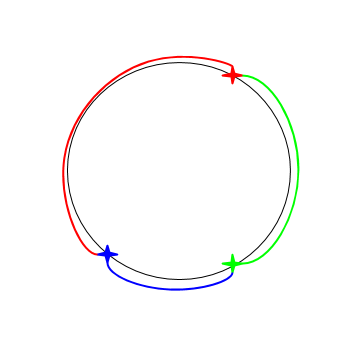
\includegraphics[width=0.3\linewidth]{figs/voro-chord-normal}
	\caption{A Voronoi diagram for a Chord network, using Chord's definition of closest.}
	\label{fig:voro-chord-normal}
\end{figure}

\begin{figure}
	\centering
	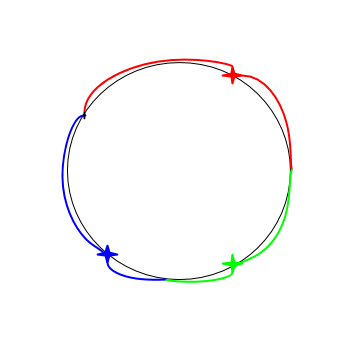
\includegraphics[width=0.5\linewidth]{figs/voro-chord-alternative}
	\caption{A Voronoi diagram for a Chord network, where closest if defined by the node being the closest in either direction.}
	\label{fig:voro-chord-alternative}
\end{figure}

 
\subsection{Terminology}
% % %unified terminology
The large number of DHTs have lead many papers use different terms to describe congruent elements of DHTs, as some terms may make sense only in one context.
Since this paper will cover multiple DHTs that would use different terms,  we have created a unified terminology:


\begin{enumerate}
    \item[key] -  The identifier generated by a hash function corresponding to a unique\footnote{Unique with extremely high probability.     The probability of a hash collision is extremely low.} node or file.
    SHA-1, which generates 160-bit hashes, is typically used as a hashing algorithm.\footnote{Due to the research into hash collisions \cite{stevens2012attacks}, and the glut of hardware that currently exists to perform SHA hash collisions, SHA1 is being depreciated by 2017.}
    
	\item[ID] - The ID is a key that corresponds to a particular node.  
	The ID of a node and the node itself are referred to interchangeably.
	In this paper, I try to refer to nodes by their ID and files by their keys.
	\item[Peer]  - Another active member on the network.
	For this section, we assume that all peers are different pieces of hardware.
	\item[Peerlist] -  The set of all peers that a node knows about. 
	This is sometimes referred to as the \textit{routing table}, but certain DHTs \cite{tapestry} \cite{pastry} overload the terminology.
	Any table or list of peers is a subset of the entire peerlist.
	\item[Short-hops] - The subset of peers that are ``closest/adjacent'' to the node in the keyspace, according to the DHT's metric.  
	In a 1-dimensional ring, such a Chord \cite{chord}, this is the node's \textit{predecessor(s)} and \textit{successor(s)}.
	They may also be called \textit{neighbors}.
	\item[Long-hops] - The subset of the peerlist that the node is not adjacent to.  
	These are sometimes referred to as fingers, long links, or shortcuts.
	\item[Root Node] - The node responsible for a particular key. 
	\item[Successor] -  Alternate name for the root node. 
	The successor of a node is the neighbor that will assume a nodes responsibilities if that node leaves. 
    \item[$n$ nodes] -  The number of nodes in the network.
    
\end{enumerate}

Similarly, All DHTs perform the same operations with minor variation.
\begin{enumerate}
	\item[\texttt{lookup(key)}] - This operation finds the root node of \texttt{key}.
	Almost every operation on a DHT needs to leverage the \texttt{lookup} operation in some way.
	\item[\texttt{put(key,value)}] - Stores \texttt{value} at the root node of \texttt{key}.
	Unless otherwise specified, \texttt{key} is assumed be the hashkey of \texttt{value}.
	This assumption is broken in Tapestry.
	\item[\texttt{get(key)}] - This operates like lookup, except the context is to return the value stored by a \texttt{put}.
	This is a subtle difference, since one could \texttt{lookup(key)} and ask the corresponding node directly.
	However, many implementations use backup operations and caching which will store multiple copies of the value along the network.
	If we do not care which node returns the value mapped with \texttt{key}, or if it is a backup,  we can express it with \texttt{get}.
	\item[\texttt{delete(key, value)}] - This is self-explanatory.  Typically, DHTs do not worry about key deletion and leave that option to the specific application.
    When DHTs do address the issue, they often assume that stored key-value pairs have a specified time-to-live, after which they are automatically removed.
\end{enumerate}

On the local level, each node has to be able to \textit{join }and perform maintenance on itself.
\begin{enumerate}
	\item[\texttt{join()}]  The join process encompasses two steps.
    First, the joining node needs to initialize its peerlist. 
    It does not necessarily need a complete peerlist the moment it joins, but it must initialize one. 
    Second, the joining node needs to inform other nodes of its existence.
    \item[Maintenance]  Maintenance procedures generally are either \textit{active} or \textit{lazy}.
    In active maintenance, peers are periodically pinged and are replaced when they are no longer detected.
    Lazy maintenance assumes that peers in the peerlist are healthy until they prove otherwise, in which case they are either replaced immediately.
    In general, lazy maintenance is used on everything, while active maintenance is only used on neighbors\footnote{check this statement for consistency}.
    
\end{enumerate}

When analyzing the DHTs in this chapter, we look at the overlay's geometry, the peerlist, the \texttt{lookup} function, and how fault-tolerance is performed in the DHTs.
We assume that nodes never politely leave the network but always abruptly fail, since a \texttt{leave()} operation is fairly trivial and has minimal impact.


\section{Chord}
%Chord \cite{chord} is a P2P protocol for file sharing and distributed storage that guarantees a high probability $\log_{2} n$ lookup time for a particular node or file in the network. 
%It is highly fault-tolerant to node failures and churn, the constant joining and leaving of nodes.  It scales extremely well and the network requires little maintenance to handle individual nodes.  



Chord \cite{chord} is the archetypal ring-based DHT and it is impossible to create a new ring-based DHT without making some comparison to Chord.
It is notable due its straightforward routing, its rules which make ownership of keys very easy to sort out, and the large number of derivatives.



% Should I put this in?
Chord is extremely famous in Computer Science, and was awarded the prestigious 2011 SIGCOMM Test of Time Award \cite{zave2012using}.
However, recent research has demonstrated that there have been no correct implementation of Chord in over a decade \cite{zave2012using}.




\subsection*{Peerlist and Geometry}
Chord is a 1-dimensional modular ring in which all messages travel in one direction - upstream, hopping from one node to another node with a greater ID until it wraps around.
Each member of the network and the data stored within it is hashed to a unique $m$-bit key or ID, corresponding to one of the $2^m$ locations on a ring. 
An example Chord network is shown in Figure \ref{fig:chord}.



\begin{figure}
	\centering
	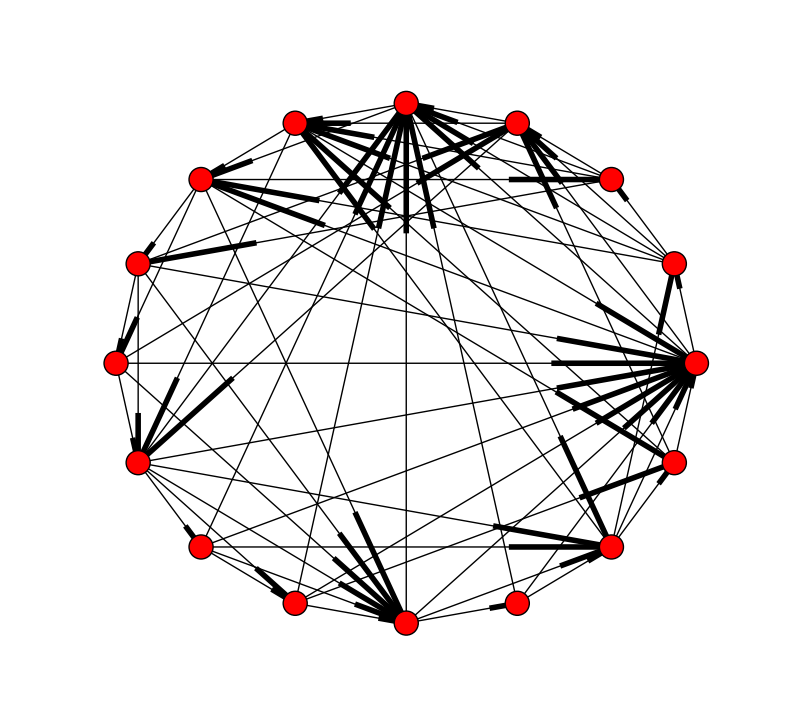
\includegraphics[width=0.45\linewidth]{figs/chord}
	\caption{A Chord ring with 16 nodes.  The fingers (long hop connections) are shown cutting across the ring.}
	\label{fig:chord}
\end{figure}



A node in the network is responsible for all the data with keys upstream from its predecessor's ID, up through and including its own ID.  
If a node is responsible for some key, it is referred to being the root or successor of that key.

Lookup and routing is performed by recursively querying nodes upstream.
Querying only neighbors in this manner would take $O(n)$ time to lookup a key.


To speedup lookups, each node maintains a table of $m$ shortcuts to other peers, called the \textit{finger table}.
The $i$th entry of a node $n$'s finger table corresponds to the node that is the successor of the key $n+2^{i-1} \mod 2^m $.  
During a lookup,  nodes query the finger that is closest to the sought key without going past it, until it is received by the root node.
Each hop essentially cuts the search space for a key in half.
This provides Chord with a highly scalable $\log_2(n)$ lookup time for any key \cite{chord}, with an average $\frac{1}{2}O(\log_{2}(n))$ number of hops.

Besides the finger tables, the peerlist includes a list of $s$ neighbors in each direction for fault tolerance.
This brings the total size of the peerlist to $log_{2}(2^{m})  + 2 \cdot s =  m  + 2 \cdot s$, assuming the entries are distinct.

\subsection*{Joining}
To join the network, node $n$ first asks $n'$ to find \texttt{successor($ n $)}. 
Node $n$ uses the information to set his successor, and maintenance will inform the other nodes of $n$'s existence.
Meanwhile, $n$ will takeover some of the keys that his successor was responsible for.

\subsection*{Fault Tolerance}
Robustness in the network is accomplished by having nodes backup their contents to their $s$ immediate successors, the closest nodes upstream. 
This is done because when a node leaves the or fail, the most immediate successor would be responsible for the keys.
In the case of multiple nodes failing all at once, having a successor list makes it extremely unlikely that any given stored value will be lost.

As nodes enter and leave the ring, the nodes use their maintenance procedures to guide them into the right place and repair any links with failed nodes.  
The process takes $O(\lg^{2}(n))$ messages.
Full details on Chord's maintenance cycle can be found here \cite{chord}.

%\subsection*{Security}
%An Eclipse attack compromises a DHT by poisoning the routing tables of nodes, such that friendly nodes can only communicate with malicious nodes \cite{dhtsec}.
%Because 





\section{Kademlia}
Kademlia \cite{kademlia}  is perhaps the most well known and definately the most widely DHT, as a modified version of Kademlia (Mainline DHT) is useds as the backbone of the Bittorrent protocol.
The motivation of Kademlia was to create a way for nodes to incorporate peerlist updates with each query made.

%(the security ramifications of gossip based routing tables being ignored, I suppose).

\subsection*{Peerlist and Geometry}
Like Chord, Kademlia uses $m$-bit keys for nodes and files.
However, Kademlia utilizes a binary tree-based structure, with the nodes acting as the leaves of the tree.
Distance between any two nodes in the tree  is calculated by XORing their IDs.
The XOR distance metric means that distances are symmetric, which is not the case in Chord.

%A node's location in the tree given by the shortest unique prefix of its ID.   
%For each bit in the prefix, there would be a subtree which does not contain that node.  
%Kademlia guarantees that the node will know at least one node in each of these subtrees.

Nodes in Kademlia maintain information about the network using a routing table that contains  $m$ lists, called $k$-buckets.
For each $k$-bucket contains up to $k$ nodes that are distance $2^i$ to $2^{i+1}$, where $0 \leq i < m$.
In other words, each $k$-bucket corresponds to a subtree of the network not containing the node.
An example network is shown in Figure \ref{fig:kademlia}.

\begin{figure}
	\centering
	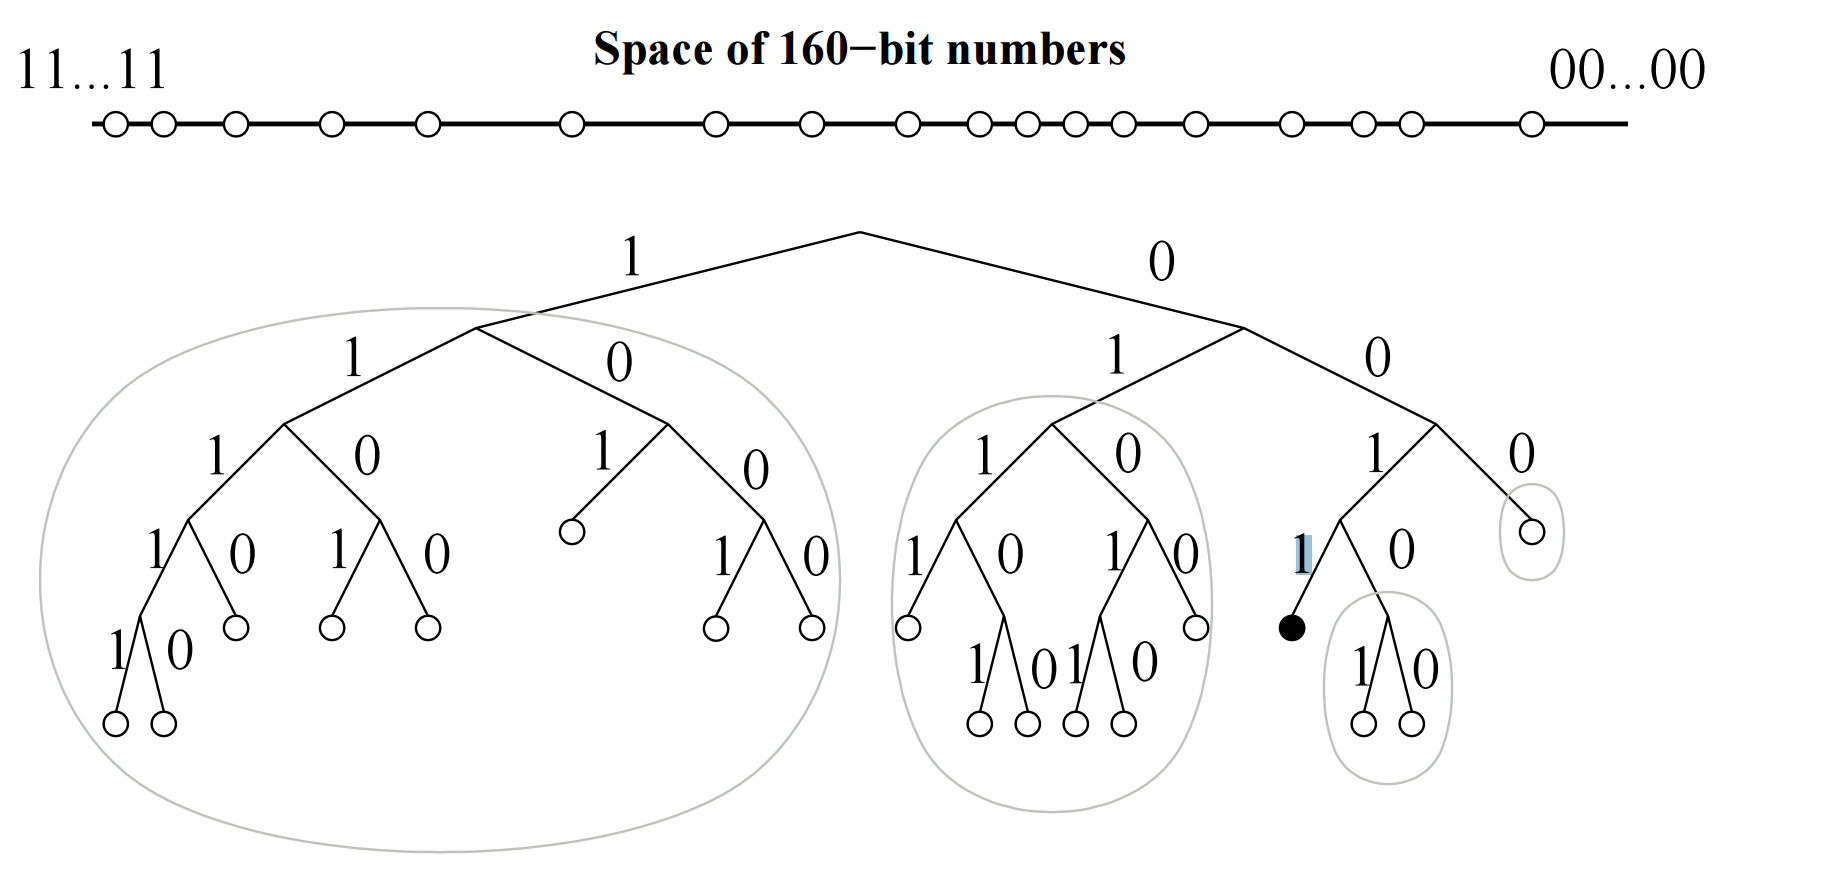
\includegraphics[width=0.7\linewidth]{figs/kademlia}
	\caption{An example Kademlia network from the original paper \cite{kademlia}. The ovals are the node's $k$-buckets.}
	\label{fig:kademlia}
\end{figure}




Each $k$-bucket is maintained by a least recently seen eviction algorithm that skips live nodes.
Whenever the node receives a message, it adds the sender's info to the tail of the corresponding $k$-bucket.
If that info already exists, the info is moved to the tail.

If the $k$-bucket is full, the node starts pinging nodes in the list, starting at the head.
As soon as a node fails to respond, that node is evicted from the list to make way for the new node at the tail.

If there are no modifications to a particular $k$-bucket after a long period of time, the node does a \texttt{refresh} on the $k$-bucket.
A refresh is a \texttt{lookup} of a random key in that $k$-bucket.


%(If I'm an eclipse attacker, I just keep spamming messages of different IDs, but with my own ip address and port info, or with sybils)

\subsection*{Lookup}
In most DHTs, \texttt{lookup(key)} sends a single message and returns the information  of a single node.
The \texttt{lookup} operation in Kademlia differs in both respects:  \texttt{lookup} is done in parallel and each node receiving  a \texttt{lookup(key)} returns the $k$ closest nodes to \texttt{key} it knows about.


A \texttt{lookup(key)} operation begins with the seeking node sending lookups in parallel to the $\alpha$ nodes from the appropriate $k$-bucket.
Each of theses $\alpha$ nodes will asynchronously return the $k$ closest nodes it knows closest to \texttt{key}.
As lookups return their results, the node continue to send lookups until no new nodes\footnote{If a file being stored on the network is the objective, the \texttt{lookup} will also terminate if a node reports having that file.} are found.  

\footnote{I would argue that this lookup operation is not recursive as claimed by the paper, but iterative, since the initiator sends all the messages.}

\subsection*{Joining}
A joining node starts with a single contact and then performs a \textit{lookup} operation on it's own ID.
Each step of the \textit{lookup} operation yields new nodes for the joining node's peerlist and informs other nodes of its existence.
Finally, the joining node performs a \texttt{refresh} on each $k$-bucket farther away than the closest node it knows of.




\subsection*{Fault-Tolerance}
Nodes actively republish each file stored on the network each hour by rerunning the \texttt{store} command.  
To avoid flooding the network, two optimizations are used.

First if a node receives a \texttt{store} on a file it is holding, it assumes $k-1$ other nodes got that same command and resets the timer for that file.
This means only one node republishes a file each hour.
Secondly, \texttt{lookup} is not performed during a republish.


Additional fault tolerance is provided by the nature of the \texttt{store(data)} operation, which \texttt{puts }the file in the $k$ closest nodes to the key.
However, there's very little in the way of frequent and active maintenance other than what occurs during \texttt{lookup} and the other operations.


%\subsubsection*{Caching}
%Files are cached during a \texttt{get} operation and stored at the closest node that the seeker found that did not return a result.
%The cache has an expiration 










\section{CAN}
%TODO: REREAD, APPARENTLY A COUPLE OF WAYS TO define NEIGHBORHOOD


Unlike the previous DHTs presented in this chapter, the Content Addressable Network (CAN) \cite{can} works in a $d$-dimensional torus, with the entire coordinate space divided among members.
A node is responsible for the keys  that fall within the ``zone'' that it owns.
Each key is hashed into some point within the geometric space.

\subsection*{Peerlist and Geometry}
CAN uses an exceptionally simple peerlist consisting only of neighbors.  
Every node in the CAN network is assigned a geometric region in the coordinate space and each node maintains a routing table consisting each node that borders the node's region.
An example CAN network is shown in \ref{fig:can}


\begin{figure}
	\centering
	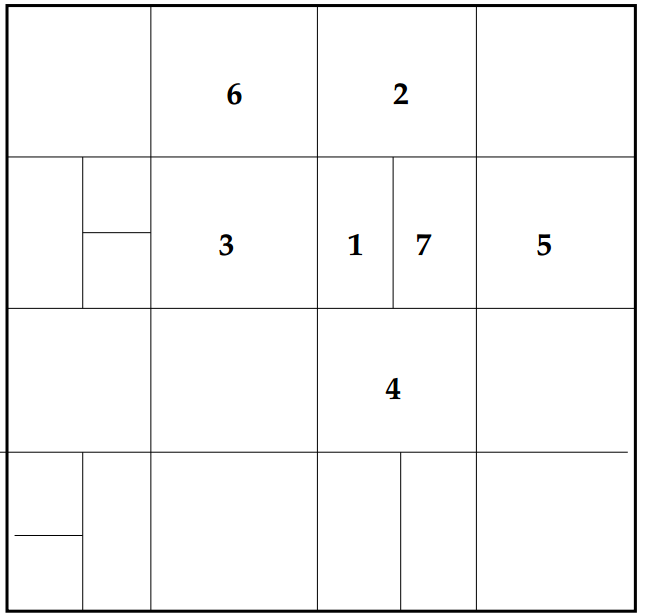
\includegraphics[width=0.7\linewidth]{figs/can}
	\caption{An example CAN network from \cite{can}.}
	\label{fig:can}
\end{figure}


The size of the routing table is a function of the number of dimensions, $O(d)$. 
The lower bound on the routing tables size in a populated network (eg, a network with at least $2d$ nodes) is $\Omega(2d)$.  
This is obtained by looking at each axis, where there is at least one node bordering each end of the axis.
The size of the routing table can grow as more nodes join and the space gets further divided; however, maintenance algorithms prevent the regions from becoming too fragmented.


\subsection*{Lookup}
As previously mentioned, each node maintains a routing table corresponding to their neighbors, those nodes it shares a face with.
Each hop forwards the lookup to the neighbor closest to the destination, until it comes to the responsible node.
In a space that is evenly divided among $n$ nodes, this simple routing scheme uses only $2 \cdot d$ space while giving average path length of $\frac{d}{4}\cdot n^{\frac{1}{d}}$.
The overall lookup time of in CAN is bounded by $O(n^{\frac{1}{d}})$ hops\footnote{Around the same time CAN was being developed, Kleinberg was doing research into small world networks \cite{kleinberg2000small}.  
He proved similar properties for lattice networks with a single shortcut.  What makes this network remarkable is lack of shortcuts.}.

% fault tolerence in routing
If a node encounters a failure during lookup, the node simply chooses the next best path.
However, if lookups occur before a node can recover from damage inflicted by churn, it is possible for the greedy lookup to fail.
The fallback method is to use an expanding ring search until a candidate is found, which recommences greedy forwarding.

\subsection*{Joining}
Joining works by splitting the geometric space between nodes.  
If node $n$ with location $P$ wishes to join the network, it contacts a member of the node to find the node $m$ currently responsible for location $P$.
Node $n$ informs $m$ that it is joining and they divide $m$'s region such that each becomes responsible for half.

Once the new zones have been defined, $n$ and $m$ create its routing table from $m$ and its former neighbors.
These nodes are then informed of the changes that just occurred and update their tables.
As a result, the join operation affects only $O(d)$ nodes.  
More details on this splitting process can be found in CAN's original paper \cite{can}.

\subsection*{Repairing}
A node in a DHT that notifies its neighbors that its leaves usually has minimal impact to the  network and in this is true for most cases in CAN.
A leaving node, $f$, simply hands over its zone to one of its neighbors of the same size, which merges the two zones together.
Minor complications occur if this is not possible, when there is no equally-sized neighbor. 
In this case, $f$ hands its zone to its smallest neighbor, who must wait for this fragmentation to be fixed.



Unplanned failures are also relatively simple to deal with.
Each node broadcasts a heartbeat to its neighbors, containing its and its neighbors' coordinates.
If a node fails to hear a heartbeat from $f$ after a number of cycles, it assumes $f$ must have failed and begins a \texttt{takeover} countdown.
When this countdown ends, the node broadcasts\footnote{This message is sent to all of $f$'s neighbors;  I assume that nodes must keep track of their neighbors' neighbors.} a \texttt{takeover} message in an attempt to claim $f$'s space.
This message contains the node's volume.
When a node receives a \texttt{takeover} message, it either cancels the countdown or, if the node's zone is smaller than the broadcaster's, responds with its own \texttt{takeover}.

The general rule of thumb for node failures in CAN is that the neighbor with the smallest zone takes over the zone of the failed node.
This rule leads to quick recoveries that affect only $O(d)$ nodes, but requires a zone reassignment algorithm to remove the fragmentation that occurs from \texttt{takeovers}.

To summarize, a failed node is detected almost immediately, and recovery occurs extremely quickly, but fragmentation must be fixed by a maintenance algorithm.




%As mentioned earlier in the text, Ratnasamy et al. \cite{can}  also present the concept own using landmarks to choose coordinates, rather than a has function.
%Each node measures the round-trip time (RTT) to each to of the $m$ landmarks, which yields one of $m!$ permutations.
%The keyspace is partitioned into $m!$ regions, each corresponding to one of the orderings.  
%A joining node now chooses a random location from the region corresponding to its landmark ordering.






%\subsection*{Design Improvements}
%Ratnasamy et al.\ identified a number of improvements that could be made to CAN \cite{can}.
%Some of these improvements have already be explored in Chapter 1.

%One modification to the system is increasing the number of dimensions in the coordinate space.
%Increasing $d$ improves fault tolerance and reduces path length.

%One concept Ratnasamy et al.\  introduces is the idea of multiple coordinate spaces existing simultaneously, called \textit{realities}. 
%Each object in the DHT exists at a different set of coordinates for each reality simultaneously.
%So a node might have coordinates $(x_0,y_0,z_0)$ in one reality, while having coordinates $(x_1,y_1,z_1)$ in another.
%Independent sets of neighbors for each reality yield different the overall topologies and mappings of keys to nodes.
%Multiple realities increase the cost of maintenance and routing table sizes, but provide greater fault tolerance and greater data availability.

%A final modification is to allow multiple nodes shares the same zone (ie zones don't necessarily split as a result of a join operation).    


\section{Pastry}

%Addressing - 128 bit ID, 0 to $2^{128} -1$, assigned randomly using hash.   but thought of as base $2^{b}$ numbers (typically b=4).  
Pastry \cite{pastry} and Tapestry \cite{tapestry} are extremely similar use a prefix-based routing mechnism introduced by Plaxton et al.\ \cite{plaxton1999accessing}.
In Pastry and Tapestry, each key is encoded as a base $ 2^{b} $ number (typically $b=4$ in Pastry, which yields easily readable hexadecimal).
The resulting peerlist best resembles a hypercube topology \cite{induced}, with each node being a vertice of the hypercube.

One notable feature of Pastry is the incorperation of a proximity metric.
The peerlist uses IDs that are close to the node according to this metric.

\subsection*{Peerlist}
Pastry's peerlist consists of three components: the routing table, a leaf set, and a neighborhood set.  
The routing table consists of $\log_{2^{b}}(n)$ rows with $2^{b} -1 $ entries per row. 
The $i$th level of the routing table correspond to the peers with that match first $i$ digits of the example nodes ID.

Thus, the 0th row contains peers which don't share a common prefix with the node, the 1st row contains those that share a length 1 common prefix, the 2nd a length 2 common prefix, etc.  
Since each ID is a base $2^b$ number, there is one entry for each of the $2^{b} -1 $ possible differences.   

For example, let is consider a node 05AF in system where $b = 4$ and the hexadecimal keyspace ranges from $0000$ to FFFF.
\begin{itemize}
    \item 1322 would be an appropriate peer for the 1st entry of level 0.
    \item 0AF2 would be an appropriate peer for the 10th\footnote{0 is the 0th level.  It's easier that way.} entry of level 1.
    \item 09AA would be an appropriate peer for the 9th entry of level 1.	
    \item 05F2 would be an appropriate peer for the 2nd entry of level 3.
\end{itemize}


The leaf set is used to hold the $L$ nodes with the numerically closest IDs;  half of it for smaller IDs and half for the larger.
A typical value for $L$ is $2^b$ or $2^{b+1}$.
The leaf set is used for routing when the destination key is close to the current node's ID.
The neighborhood set contains the $L$ closest nodes, as defined by some proximity metric.  
It, however, is generally not used for routing.  
Figure \ref{fig:pastry-table} shows an example peerlist of a node in PAST.

\begin{figure}
	\centering
	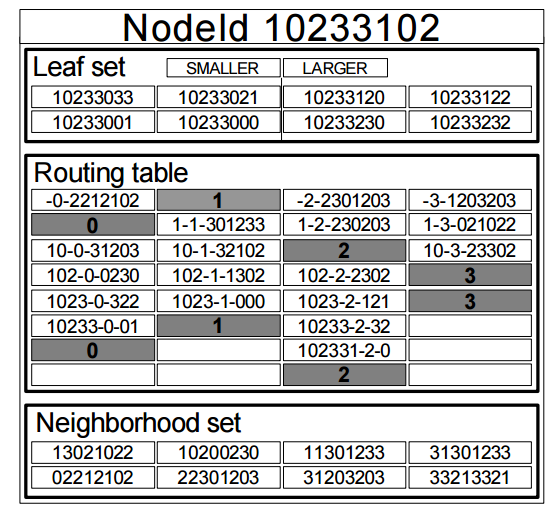
\includegraphics[width=0.5\linewidth]{figs/pastry-table}
	\caption{An example peerlist for a node in Pastry. Taken from the original Pastry paper \cite{pastry}.}
	\label{fig:pastry-table}
\end{figure}



\subsection*{Lookup}
The \texttt{lookup} operation is a fairly straightforward recursive operation.
The \texttt{lookup(key)} terminates when the \texttt{key} is falls within the range of the leaf set, which are the nodes \emph{numerically} closest to the current node.
In this case, the destination will be one of the leaf set, or the current node.

If the destination node is not immediately apparent, the node uses its routing table to select the next node.
The node looks at the length $l$ shared prefix,  at examines the $l$th row of its routing table.
From this row, the \texttt{lookup} continues with the entry that matches at least another digit of the prefix.
In the case that this entry does not exist or has failed, the \texttt{lookup} continues from the closest ID chosen from the entire peerlist.
This process is described by Algorithm \ref{PastryLookup}.
Lookup is expected  to take $\lceil \log_{2^{b}} \rceil $, as each hop along the routing table reduces the search space by $\frac{1}{2^{b}}$.
 
\begin{algorithm}
    \caption{Pastry lookup algorithm}
    \label{PastryLookup}
    \begin{algorithmic}
        \State Let $L$ be the routing  
        \Function{Lookup}{$key$}
            \If {$key$ is in the range of the leaf set }
            	\State destination is closest ID in the leaf set or self
            \Else
            	\State $next\gets$ entry from routing table that matches $\geq 1$ more digit
            	\If {$next \neq null$}
                	\State forward to $next$
            	\Else
                	\State forward to the closest ID from the entire peerlist
                \EndIf
                
            \EndIf
        \EndFunction
    \end{algorithmic}
\end{algorithm}

\subsection*{Joining}
To join the network, node $J$ sends a \texttt{join} message to $A$, some node that is close according to the proximity metric.
The \texttt{join} message is forwarded along like a \texttt{lookup} to the root of $X$, which we'll call $root$.
Each node that received the \texttt{join} sends a copy of the their peerlist to $J$.

The leaf set is constructed from copying $root$'s leaf set, while $i$th row in the routing table routing table is copied from the $i$th node contacted along the \texttt{join}.
The neighborhood set is copied from $A$'s neighborhood set, as \texttt{join} predicates that $A$ be close to $J$.
This means $A$'s neighborhood set would be close to $A$. 

After the joining node creates its peerlist, it sends a copy to each node in the table, who then can update their routing tables.  
The cost of a \texttt{join} is $O(log_{2}^{b} n)$ messages,  with  a constant  coefficient  of $3*2^{b}$




\subsection*{Fault Tolerance}
Pastry lazily repairs its leaf set and routing table.
When node from the leaf set fails, the node contacts the node with largest or smallest ID (depending if the failed node ID was smaller or larger respectively) in the leaf set.
That node returns a copy of its leaf set, and the node replaces the failed entry.
If the failed node is in the routing table, the node contacts a node with an entry in the same row as the failed node for a replacement.

Members of the neighborhood set are actively checked.
If a member of the neighborhood set is unresponsive, the node obtains a copy of another entry's neighborhood set and repairs from a selection.



%\subsection*{Proximity Metric}
%Pastry's goal is to minimize the ``distance'' messages travel, where distance can be defined by some metric, typically the number of hops.
%The leaf set is the  of nodes closest to the node in the keyspace.  
%The neighborhood set is the of nodes closest to the node according to the distance metric. 
%Guarantees routing time is  $<\log n$ in typical operation.  
%Guarantees eventual delivery except when half of the leaf nodes fail simultaneously.






%\section{Tapestry}
%Tapestry \cite{tapestry} is based off the same prefix-based lookup \cite{prr} as Pastry \cite{pastry} and the peerlist and lookup operation share many similarities.
%Tapestry views itself more as a DOLR \cite{dolr}.
%This essentially means that it is a distributed key-based lookup system like a DHT \cite{hildrum2004distributed}, but with some subtle differences at the abstract level which manifest as large %implementation changes.
%The essential difference here is that Tapestry has servers \textit{publish} records/objects on the network, which direct lookups to the server.  
%The assumption here seems to be that the servers, not the responsible node, serve the actual data.  
%DHTs care or don't care on an application to application basis whether keys are associated with records or content. 






% ``Small'' routing tables
\section{Symphony and Small World Routing}
Symphony  \cite{symphony} is a 1$d$ ring-based DHT similar to Chord \cite{chord}, but is constructed using the properties of small world networks \cite{kleinberg2000small}.
Small world networks owe their name to a phenomena observed by psychologists in the late 1960's. 

Subjects in experiments were to route a postal message to a target person; for example the wife of a Cambridge divinity student in one experiment and a Boston stockbroker in another \cite{milgram1967small}.
The messages were only to be routed by forwarding them to a friend they thought most likely to know the target.
Of the messages that successfully made their way to the destination, the average path length from a subject to a participant was only 5 hops.  

This lead to research investigating creating a network with randomly distributed links, but with a efficient lookup time.
Kleinberg \cite{kleinberg2000navigation} showed that in a 2-dimensional lattice network, nodes could route messages in $O(\log^{2}n)$ hops using only their neighbors and a single randomly chosen\footnote{Randomly chosen from a specified distribution.} finger.
In other words, $O(\log^{2}n)$ lookup is achievable with a $O(1)$ sized routing table.

\subsection*{Peerlist}
Rather than the 2-dimensional lattice used by Kleinberg, Symphony uses a 1-dimensional ring\footnote{This is technically a 1-dimensional lattice.} like Chord.
Symphony assigns $m$-bit keys to the modular unit interval $ [0,1)$, instead of using a keyspace ranging from 0 to $2^{n} - 1$.
This location is found  with $\frac{hashkey}{2^{m}}$.
This is arbitrary from a design standpoint, but makes choosing from a random distribution simpler. 

Nodes know both their immediate predecessor and successor, much like in Chord.
Nodes also keep track of some  $k \geq 1$ fingers, but, unlike in Chord, these fingers are chosen at random.
These fingers are chosen from a probability distribution corresponding to the expression $e^{ln(n) + (rand48() - 1.0)}$, where $n$ is the number of nodes in the network and \texttt{rand48()} is a C function that generates a random float?double between 0.0 and 1.0.
Because $n$ os difficult to compute due to the changing nature of P2P networks, each node uses an approximation is used based on the distance between themselves and their neighbors.

A final feature of note is that links in Symphony are bidirectional.
Thus, if a node creates a finger to a peer, that peer creates a, so nodes in Symphony have a grand total of $2k$ fingers.
%(although it gets me thinking, is there any advantage/statistical properties   that could be exploited by making the space monic)


\subsection*{Joining and Fault Tolerance}
The joining and fault tolerance processes in Symphony are extremely straightforward.
After determining its ID, a joining node asks a member to find the root node for its ID.
The joining node integrates itself in between its predecessor and successor and then randomly generates its fingers.

Failures of immediate neighbors are handled by use of successor and predecessor lists
Failures for fingers are handled lazily and are replaced by another randomly generated link when a failure is detected.

% Large Routing Tables
\section{ZHT}
One of the major assumptions of DHT design is that churn is a significant factor, which requires constant maintenance to handle.
A consequence of this assumption is that nodes only store a small subset of the entire network to route to.
Storing the entire network is not scalable for the vast majority of distributed systems due to bandwidth constraints and communication overhead incurred by the constant joining and leaving of nodes.

In a system that does not expect churn, the memory and bandwidth costs for each node to keep a full copy of the routing table are minimal.
An example of this would be a data center or a cluster built for higher-performance computing, where churn would overwhelmingly be the result of hardware failure, rather than users quitting.

ZHT \cite{li2013zht} is an example of such a system, as is Amazon's Dynamo \cite{dynamo}.
ZHT is a ``zero-hop hash table,'' which takes advantage of the fact that  nodes in  High-End Computing environments have a predictable lifetime.
Nodes are created when a job begins and are removed when a job ends.
This property allows ZHT to \texttt{lookup} in $ O(1) $ time.

\subsection*{Peerlist}

ZHT operates in a 64-bit ring, for a total of $N = 2^{64}$ addresses.
ZHT places a  hard limit of $ n $ on the maximum number of physical nodes in the network, which means the network has $n$ partitions of $\frac{N}{n} =  \frac{2^{64}}{n}$ keys.
The partitions are evenly divided along the network.

The network consists of $k$ physical nodes which each are running at least one instance (virtual nodes) of ZHT, with a combined total of $i$ .
Each instance is responsible for some span of partitions in the ring.


Each node maintains a complete list of all nodes in the network, which do not have to be updated very often due to the lack of or very low levels of churn.
The memory cost is extremely low.
Each instance has a 10MB footprint, and each entry for the membership table takes only 32 bytes per node.
This means routing takes anywhere between 0 to 2 hops (explained below).

\subsection*{Joining}
ZHT operates under a static or dynamic membership.
In a static membership, no nodes will be joining the network once the network has been bootstrapped.
Nodes can join at any time when ZHT is using dynamic membership.

To join, the joiner asks a random member for a copy of the peerlist 
The joiner can then determine which node is the most heavily overloaded.
The joiner chooses an address in the network to take over partitions from that node.


No idea how membership table is updated

\subsection*{Fault Tolerance}
Fault tolerance exists to handle only hardware failure or planned departures from the network.
Nodes backup their data to their neighbors.


\section{VHash}
DHTs all seek to minimize lookup time for their respective topologies.
This is done by minimizing the number of overlay hops needed for a lookup operation.
This is a good approximation for minimizing the latency of lookups, but does not actually do so.
Furthermore, a network might need to minimize some arbitrary metric, such as energy consumption.

VHash is a multi-dimensional DHT that minimizes routing over some given metric.
It uses a fast approximation of a Delaunay Triangulation to compute the Voronoi tessilation of a multi-dimensional space.
%Approximated routing tables



Arguably all Distributed Hash Tables (DHTs) are built on the concept of Voronoi tessellation.
In all DHTs, a node is responsible for all points in the overlay to which it is the ``closest'' node.
Nodes are assigned a key as their location in some keyspace, based on the hash of certain attributes.
Normally, this is just the hash of the IP address (and possibly the port) of the node \cite{chord} \cite{kademlia} \cite{can} \cite{pastry}, but other metrics such as geographic location can be used as well \cite{ratnasamy2002ght}.

These DHTs have carefully chosen metric spaces such that these regions are very simple to calculate.
For example, Chord \cite{chord} and similar ring-based DHTs \cite{manku2003symphony} utilize a unidirectional, one-dimensional ring as their metric space, such that the region for which a node is responsible is the region between itself and its predecessor.

Using a Voronoi tessellation in a DHT generalizes this design. 
Nodes are Voronoi generators at a position based on their hashed keys.
These nodes are responsible for any key that falls within its generated Voronoi region.

Messages get routed along links to neighboring nodes. 
This would take $O(n)$ hops in one dimension.
In multiple dimensions, our routing algorithm (Algorithm \ref{alg:lookup}) is extremely similar to the one used in Ratnasamy et al.'s Content Addressable Network (CAN) \cite{can}, which would be $O(n^{\frac{1}{d}})$ hops.


\begin{algorithm}
	\caption{Lookup in a Voronoi-based DHT}
	\label{alg:lookup}
	\begin{algorithmic}[1] 
		\State Given node $n$
		\State Given $m$ is a message addressed for $loc$
		\State $potential\_dests \leftarrow n \cup n.short\_peers \cup n.long\_peers$
		\State $c \leftarrow $ node in $ potential\_dests$ with shortest distance to $loc$
		\If{$c$ == $n$}
			\State \Return $n$
		\Else 
			\State \Return $c.lookup(loc)$
		\EndIf
	\end{algorithmic}
\end{algorithm}


Efficient solutions, such as Fortune's sweepline algorithm \cite{fortune1987sweepline}, are not usable in spaces with 2 more dimensions.
As far as we can tell, there is no way efficient to generate higher dimension Voronoi tessellations, especially in the distributed Churn-heavy context of a DHT.
Our solution is the Distributed Greedy Voronoi Heuristic.

\subsection*{Distributed Greedy Voronoi Heuristic}
A Voronoi tessellation is the partition of a space into cells or regions along a set of objects $O$, such that all the points in a particular region are closer to one object than any other object.  
We refer to the region owned by an object as that object's Voronoi region.
Objects which are used to create the regions are called Voronoi generators.
In network applications that use Voronoi tessellations, nodes in the network act as the Voronoi generators.

The Voronoi tessellation and Delaunay triangulation are dual problems, as an edge between two objects in a Delaunay triangulation exists if and only if those object's Voronoi regions border each other.  
This means that solving either problem will yield the solution to both.   
An example Voronoi diagram is shown in Figure \ref{voro-ex}.
For additional information, Aurenhammer \cite{voronoi} provides a formal and extremely thorough description of Voronoi tessellations, as well as their applications.


\begin{figure}
	\centering
	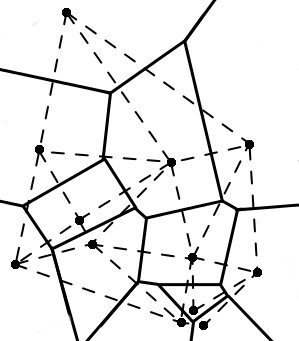
\includegraphics[width=0.5\linewidth]{figs/voronoi}
	\caption{An example Voronoi diagram for objects on a 2-dimensional space.  The black lines correspond to the borders of the Voronoi region, while the dashed lines correspond to the edges of the Delaunay Triangulation.}
	\label{voro-ex}
\end{figure}




The Distributed Greedy Voronoi Heuristic (DGVH) is a fast method for nodes to define their individual Voronoi region (Algorithm \ref{alg:dgvh}). 
This is done by selecting the nearby nodes that would correspond to the points connected to it by a Delaunay triangulation.
The rationale for this heuristic is that, in the majority of cases, the midpoint between two nodes falls on the common boundary of their Voronoi regions.

%In addition, nodes should only have to compute their own Voronoi region, and possibly estimate those of its neighbors. 
%Anything else is a waste of processing power.



\begin{algorithm} % make smaller
	\caption{Distributed Greedy Voronoi Heuristic}
	\label{alg:dgvh}
	\begin{algorithmic}[1]  % the numberis how many lines
		\State Given node $n$ and its list of $candidates$.
		\State Given the minimum $table\_size$
		\State $short\_peers \leftarrow$ empty set that will contain $n$'s one-hop peers
		\State $long\_peers \leftarrow$ empty set that will contain $n$'s two-hop peers    
		\State Sort $candidates$ in ascending order by each node's distance to $n$
		\State Remove the first member of $candidates$ and add it to $short\_peers$
		\ForAll{$c$ in $candidates$}
		\State $m$ is the midpoint between $n$ and $c$
		\If{Any node in $short\_peers$ is closer to $m$ than $n$}
		\State Reject $c$ as a peer
		\Else
		\State Remove $c$ from $candidates$
		\State Add $c$ to $short\_peers$
		\EndIf
		\EndFor
		\While{$|short\_peers| < table\_size$ \textbf{and} $|candidates| >0$}
		\State Remove the first entry $c$ from $candidates$
		\State Add $c$ to $short\_peers$
		\EndWhile
		\State Add $candidates$ to the set of $long\_peers$	
		\If{$|long\_peers| > table\_size^2$}
		\State $long\_peers \leftarrow$ random subset of $long\_peers$ of size $table\_size^2$
		\EndIf
	\end{algorithmic}
\end{algorithm}


During each cycle, nodes exchange their peer lists with a current neighbor and then recalculate their neighbors.  
A node combines their neighbor's peer list with its own to create a list of candidate neighbors.
This combined list is sorted from closest to furthest.
A new peer list is then created starting with the closest candidate.
The node then examines each of the remaining candidates in the sorted list and calculates the midpoint between the node and the candidate.
If any of the nodes in the new peer list are closer to the midpoint than the candidate, the candidate is set aside.  
Otherwise the candidate is added to the new peer list.


DGVH never actually solves for the actual polytopes that describe a node's Voronoi region.
This is unnecessary and prohibitively expensive \cite{raynet}.
Rather, once the heuristic has been run, nodes can determine whether a given point would fall in its region.

Nodes do this by calculating the distance of the given point to itself and other nodes it knows about.
The point falls into a particular node's Voronoi region if it is the node to which it has the shortest distance.
This process continues recursively until a node determines that itself to be the closest node to the point.
Thus, a node defines its Voronoi region by keeping a list of the peers that bound it.



\subsubsection{Algorithm Analysis}

DVGH is very efficient in terms of both space and time.
Suppose a node $n$ is creating its short peer list from $k$ candidates in an overlay network of $N$ nodes. 
The candidates must be sorted, which takes $O(k\cdot\lg(k))$ operations.  
Node $n$ must then compute the midpoint between itself and each of the $k$ candidates.  
Node $n$ then compares distances to the midpoints between itself and all the candidates.  
This results in a cost of 

\[ k\cdot\lg(k) + k \text{ midpoints}  + k^{2} \text{ distances} \]


Since $k$ is  bounded by $\Theta(\frac{\log N}{\log \log N} )$ \cite{bern1991expected} (the expected maximum degree of a node), we can translate the above to

\[O(\frac{\log^{2} N}{\log^{2} \log N} )\]

In the vast majority of cases, the number of peers is equal to the minimum size of \textit{Short Peers}. 
This yields $k=(3d+1)^{2}+3d+1$ in the expected case, where the lower bound and expected complexities are $\Omega(1)$.


%\subsection*{Peerlist and Topology}
%Like CAN \cite{can}, VHash tracks only neighbors for it's peers.
%We enforce a lower limit on the size of the peerlist to avoid nodes being 


%\subsection*{Joining}


%\subsection*{Fault Tolerance}


\section{Summary}
% % % table
% Perhaps geometries should be included?
% be sure to include join and leave costs.

We have seen that there are a wide variety of distributed hash tables, but they have some clearly defined characteristics that bind them all together.
Table \ref{tab:tradeoffs} summarizes the information presented in this chapter.


\begin{table}[h]
	\tiny
	\centering
	\begin{tabularx}{\textwidth}{ |X|X|X|X|X| }
		\hline
		% Add join leave cost, avgerages and maxs
		DHT & Routing Table Size & Lookup Time & Join/Leave & Comments \\ \hline  
		
		Chord \cite{chord} & $O(\log n)$, maximum $m +2s$ & $O(\log n)$, avg $(\frac{1}{2} \log n)$  &  $<O(\log n^{2})$ total messages& $m$  = keysize in bits, $s$ is neighbors in 1 direction  \\ \hline
		
		Kademlia \cite{kademlia} & $O(\log n)$, maximum $m\ \cdot k$ & $(\lceil \log n\rceil) + c$ & $O(\log(n))$& This is without considering optimization   \\ \hline
		CAN \cite{can} & $\Omega(2d)$ & $O(n^{\frac{1}{d}})$, average $\frac{d}{4}\cdot n^{\frac{1}{d}}$ & Affects $O(d)$ nodes & $d$ is the number of dimensions \\ \hline
		
		Plaxton-based DHTs, Pastry \cite{pastry}, Tapestry \cite{tapestry} & $O(\log_{\beta} n)$ & $ O(\lceil \log_{2^{\beta}} \rceil) $ & $O(\log_{\beta} n)$ &  NodeIDs are base $\beta$ numbers \\ \hline
		
        Symphony \cite{symphony}& $2k + 2$&   average $O(\frac{1}{k} \log^{2} n )$ & $O(\log^{2} n)$ messages,  constant $<1$ &  $k \geq 1$, fingers are chosen at random\\ \hline  
		
        ZHT \cite{li2013zht}&   $O(n)$& $O(1)$ &  $O(n)$ & Assumes an extremely low churn \\ \hline
        
        VHash & $\Omega(3d+1) + O((3d+1)^{2})$ & $O(\sqrt[d]{n})$ hops & $3d + 1$ & approximates regions, hops are based least latency\\ \hline
	\end{tabularx}
	\caption{The different ratios and their associated DHTs}
	\label{tab:tradeoffs}
\end{table}

% % % Specific DHTs




\chapter{Completed Work}
\label{chapter:prev}
%TODO: Add in other algorithm blocks and pictures from CHRONUS paper


DHTs have received a great deal of research due to their popularity as the backbone for structured P2P system primarily used for file-sharing.
There are two recent and fairly open questions that I want to examine.

\begin{enumerate}
	\item How can DHTs effectively be used for distributed computations?  
	In what contexts is this feasible:  only in the data center, or can a large-scale worldwide P2P network be used to do distributed computation?
	Is it better to use DHTs as an organizing mechanism, or as the actual platform for computation.
	\item How can nodes autonomously load balance?
\end{enumerate}



\section{VHash}
DHTs all seek to minimize lookup time for their respective topologies.
This is done by minimizing the number of overlay hops needed for a lookup operation.
This is a good approximation for minimizing the latency of lookups, but does not actually do so.
Furthermore, a network might need to minimize some arbitrary metric, such as energy consumption.

VHash is a multi-dimensional DHT that minimizes routing over some given metric.
It uses a fast approximation of a Delaunay Triangulation to compute the Voronoi tessilation of a multi-dimensional space.
%Approximated routing tables



Arguably all Distributed Hash Tables (DHTs) are built on the concept of Voronoi tessellation.
In all DHTs, a node is responsible for all points in the overlay to which it is the ``closest'' node.
Nodes are assigned a key as their location in some keyspace, based on the hash of certain attributes.
Normally, this is just the hash of the IP address (and possibly the port) of the node \cite{chord} \cite{kademlia} \cite{can} \cite{pastry}, but other metrics such as geographic location can be used as well \cite{ratnasamy2002ght}.

These DHTs have carefully chosen metric spaces such that these regions are very simple to calculate.
For example, Chord \cite{chord} and similar ring-based DHTs \cite{symphony} utilize a unidirectional, one-dimensional ring as their metric space, such that the region for which a node is responsible is the region between itself and its predecessor.

Using a Voronoi tessellation in a DHT generalizes this design. 
Nodes are Voronoi generators at a position based on their hashed keys.
These nodes are responsible for any key that falls within its generated Voronoi region.

Messages get routed along links to neighboring nodes. 
This would take $O(n)$ hops in one dimension.
In multiple dimensions, our routing algorithm (Algorithm \ref{alg:lookup}) is extremely similar to the one used in Ratnasamy et al.'s Content Addressable Network (CAN) \cite{can}, which would be $O(n^{\frac{1}{d}})$ hops.


\begin{algorithm}
	\caption{Lookup in a Voronoi-based DHT}
	\label{alg:lookup}
	\begin{algorithmic}[1] 
		\State Given node $n$
		\State Given $m$ is a message addressed for $loc$
		\State $potential\_dests \leftarrow n \cup n.short\_peers \cup n.long\_peers$
		\State $c \leftarrow $ node in $ potential\_dests$ with shortest distance to $loc$
		\If{$c$ == $n$}
			\State \Return $n$
		\Else 
			\State \Return $c.lookup(loc)$
		\EndIf
	\end{algorithmic}
\end{algorithm}


Efficient solutions, such as Fortune's sweepline algorithm \cite{fortune1987sweepline}, are not usable in spaces with 2 more dimensions.
As far as we can tell, there is no way efficient to generate higher dimension Voronoi tessellations, especially in the distributed Churn-heavy context of a DHT.
Our solution is the Distributed Greedy Voronoi Heuristic.

\subsection*{Distributed Greedy Voronoi Heuristic}
A Voronoi tessellation is the partition of a space into cells or regions along a set of objects $O$, such that all the points in a particular region are closer to one object than any other object.  
We refer to the region owned by an object as that object's Voronoi region.
Objects which are used to create the regions are called Voronoi generators.
In network applications that use Voronoi tessellations, nodes in the network act as the Voronoi generators.

The Voronoi tessellation and Delaunay triangulation are dual problems, as an edge between two objects in a Delaunay triangulation exists if and only if those object's Voronoi regions border each other.  
This means that solving either problem will yield the solution to both.   
An example Voronoi diagram is shown in Figure \ref{voro-ex}.
For additional information, Aurenhammer \cite{voronoi} provides a formal and extremely thorough description of Voronoi tessellations, as well as their applications.


\begin{figure}
	\centering
	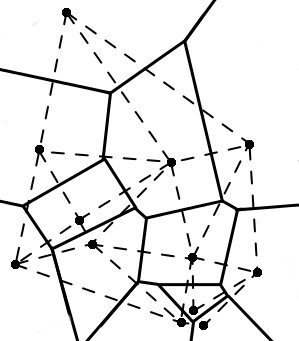
\includegraphics[width=0.5\linewidth]{figs/voronoi}
	\caption{An example Voronoi diagram for objects on a 2-dimensional space.  The black lines correspond to the borders of the Voronoi region, while the dashed lines correspond to the edges of the Delaunay Triangulation.}
	\label{voro-ex}
\end{figure}




The Distributed Greedy Voronoi Heuristic (DGVH) is a fast method for nodes to define their individual Voronoi region (Algorithm \ref{alg:dgvh}). 
This is done by selecting the nearby nodes that would correspond to the points connected to it by a Delaunay triangulation.
The rationale for this heuristic is that, in the majority of cases, the midpoint between two nodes falls on the common boundary of their Voronoi regions.

%In addition, nodes should only have to compute their own Voronoi region, and possibly estimate those of its neighbors. 
%Anything else is a waste of processing power.



\begin{algorithm} % make smaller
	\caption{Distributed Greedy Voronoi Heuristic}
	\label{alg:dgvh}
	\begin{algorithmic}[1]  % the numberis how many lines
		\State Given node $n$ and its list of $candidates$.
		\State Given the minimum $table\_size$
		\State $short\_peers \leftarrow$ empty set that will contain $n$'s one-hop peers
		\State $long\_peers \leftarrow$ empty set that will contain $n$'s two-hop peers    
		\State Sort $candidates$ in ascending order by each node's distance to $n$
		\State Remove the first member of $candidates$ and add it to $short\_peers$
		\ForAll{$c$ in $candidates$}
		\State $m$ is the midpoint between $n$ and $c$
		\If{Any node in $short\_peers$ is closer to $m$ than $n$}
		\State Reject $c$ as a peer
		\Else
		\State Remove $c$ from $candidates$
		\State Add $c$ to $short\_peers$
		\EndIf
		\EndFor
		\While{$|short\_peers| < table\_size$ \textbf{and} $|candidates| >0$}
		\State Remove the first entry $c$ from $candidates$
		\State Add $c$ to $short\_peers$
		\EndWhile
		\State Add $candidates$ to the set of $long\_peers$	
		\If{$|long\_peers| > table\_size^2$}
		\State $long\_peers \leftarrow$ random subset of $long\_peers$ of size $table\_size^2$
		\EndIf
	\end{algorithmic}
\end{algorithm}


During each cycle, nodes exchange their peer lists with a current neighbor and then recalculate their neighbors.  
A node combines their neighbor's peer list with its own to create a list of candidate neighbors.
This combined list is sorted from closest to furthest.
A new peer list is then created starting with the closest candidate.
The node then examines each of the remaining candidates in the sorted list and calculates the midpoint between the node and the candidate.
If any of the nodes in the new peer list are closer to the midpoint than the candidate, the candidate is set aside.  
Otherwise the candidate is added to the new peer list.


DGVH never actually solves for the actual polytopes that describe a node's Voronoi region.
This is unnecessary and prohibitively expensive \cite{raynet}.
Rather, once the heuristic has been run, nodes can determine whether a given point would fall in its region.

Nodes do this by calculating the distance of the given point to itself and other nodes it knows about.
The point falls into a particular node's Voronoi region if it is the node to which it has the shortest distance.
This process continues recursively until a node determines that itself to be the closest node to the point.
Thus, a node defines its Voronoi region by keeping a list of the peers that bound it.



\subsubsection{Algorithm Analysis}

DVGH is very efficient in terms of both space and time.
Suppose a node $n$ is creating its short peer list from $k$ candidates in an overlay network of $N$ nodes. 
The candidates must be sorted, which takes $O(k\cdot\lg(k))$ operations.  
Node $n$ must then compute the midpoint between itself and each of the $k$ candidates.  
Node $n$ then compares distances to the midpoints between itself and all the candidates.  
This results in a cost of 

\[ k\cdot\lg(k) + k \text{ midpoints}  + k^{2} \text{ distances} \]


Since $k$ is  bounded by $\Theta(\frac{\log N}{\log \log N} )$ \cite{bern1991expected} (the expected maximum degree of a node), we can translate the above to

\[O(\frac{\log^{2} N}{\log^{2} \log N} )\]

In the vast majority of cases, the number of peers is equal to the minimum size of \textit{Short Peers}. 
This yields $k=(3d+1)^{2}+3d+1$ in the expected case, where the lower bound and expected complexities are $\Omega(1)$.



\subsection{Experiments}
We evaluated the effectiveness of DGVH in creating an  


\subsubsection{Convergence}
Our second set of experiments examines how DGVH could be used to create a DHT and how well it would perform in this task.
Our simulation demonstrates how DGVH  can be used to create a stable overlay from a chaotic starting topology after a sufficient number of gossip cycles.  
We do this by showing that the rate of successful lookups approaches 1.0.
We compare these results to RayNet \cite{raynet}, which proposed that a random $k$-connected graph would be a good, challenging starting configuration for demonstrating convergence of a DHT to a stable network topology.

During the first two cycles of the simulation, each node bootstraps its short peer list by appending 10 nodes, selected uniformly at random from the entire network.
In each cycle, the nodes gossip (Algorithm \ref{alg:gossip}) and run DGVH using the new information.
We then calculate the hit rate of successful lookups by simulating 2000 lookups from random nodes to random locations, as described in Algorithm \ref{routesim}.
A lookup is successful when the network correctly determines which Voronoi region contains a randomly selected point.


Our experimental variables for this simulation were the number of nodes in the DGVH generated overlay and the number of dimensions.  
We tested network sizes of 500, 1000, 2000, 5000, and 10000 nodes each in 2, 3, 4, and 5 dimensions.
The hit rate at each cycle is $\frac{hits}{2000}$, where $hits$ are the number of successful lookups.




\begin{algorithm}
	\caption{Routing Simulation Sample}
	\label{routesim}
	\begin{algorithmic}[1]  % the number is how many 
		\State $start \leftarrow$ random node
		\State$dest \leftarrow$ random set of coordinates
		\State $ans \leftarrow$ node closest to $dest$
		\If {$ans == start.lookup(dest)$}
		\State increment $hits$
		\EndIf
	\end{algorithmic} 
\end{algorithm}

Our results are shown in Figures \ref{fig:conv2}, \ref{fig:conv3}, \ref{fig:conv4}, and \ref{fig:conv5} for each dimension.
Our graphs show that the created overlay quickly constructs itself from a random configuration and that our hit rate reached 90\% by cycle 20, regardless of dimension.
Lookups consistently approached a hit rate of 100\% by cycle 30. 
In comparison, RayNet's routing converged to a perfect hit rate at around cycle 30 to 35 \cite{raynet}.
As the network size and number of dimensions each increase, convergence slows, but not to a significant degree.

\begin{figure*}
	\label{fig:conv}
	\centering 
	\begin{tabular}{cc}
		
		\begin{subfigure}{0.5\columnwidth}
			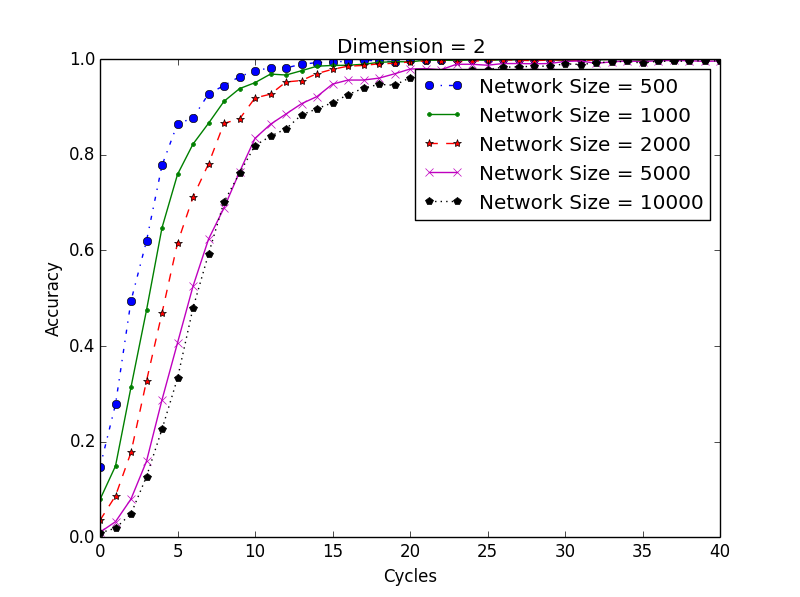
\includegraphics[width=\linewidth]{figs/conv_d2}
			\caption{This plot shows the accuracy rate of lookups on a 2-dimensional network as it self-organizes.}
			\label{fig:conv2}
		\end{subfigure} &
		
		\begin{subfigure}{0.5\columnwidth}
			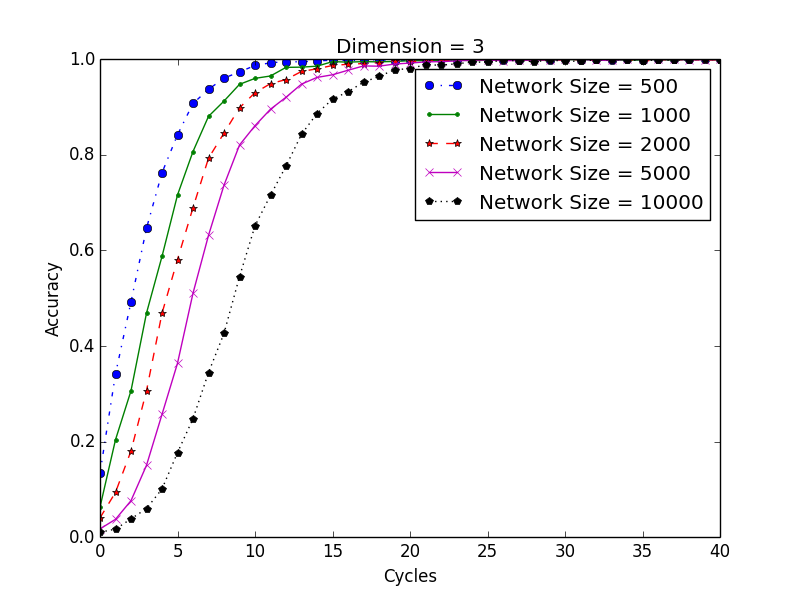
\includegraphics[width=\linewidth]{figs/conv_d3}
			\caption{This plot shows the accuracy rate of lookups on a 3-dimensional network as it self-organizes.}
			\label{fig:conv3}
		\end{subfigure} \\
		
		\begin{subfigure}{0.5\columnwidth}
			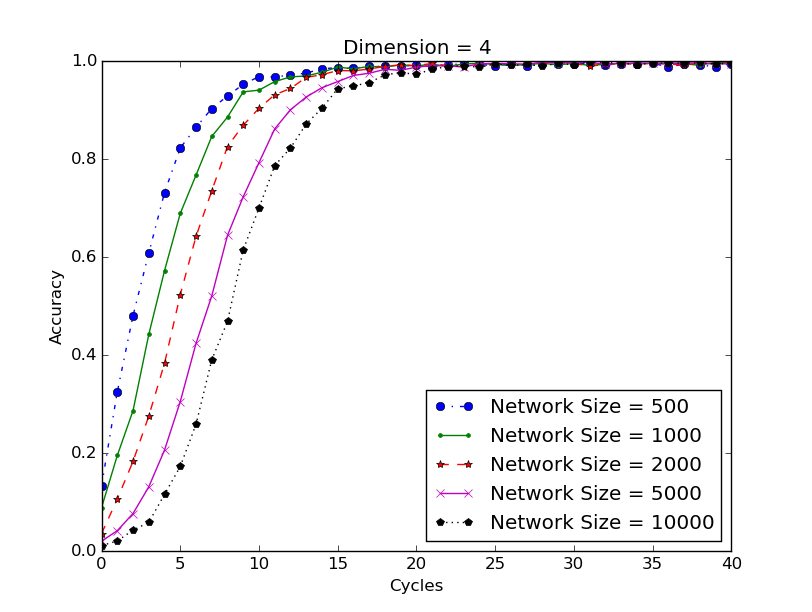
\includegraphics[width=\linewidth]{figs/conv_d4}
			\caption{This plot shows the accuracy rate of lookups on a 4-dimensional network as it self-organizes.}
			\label{fig:conv4}
		\end{subfigure} &
		
		
		\begin{subfigure}{0.5\columnwidth}
			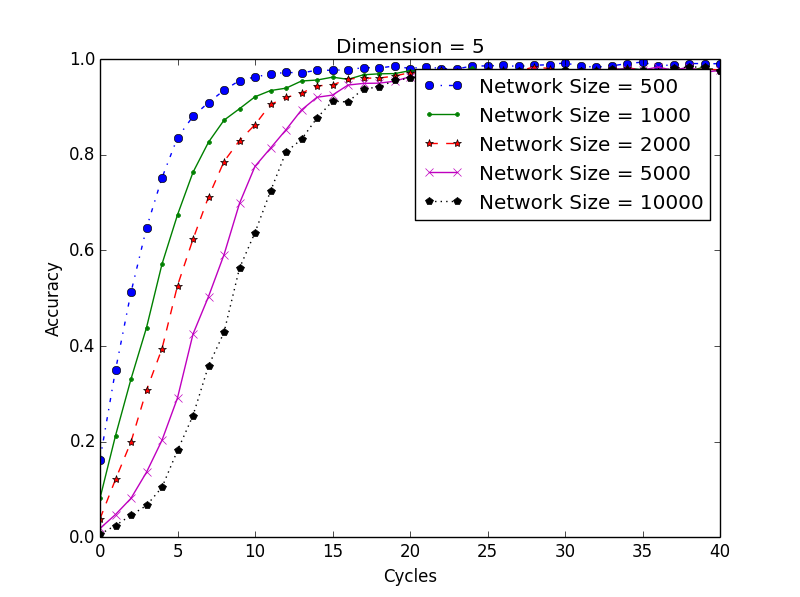
\includegraphics[width=\linewidth]{figs/conv_d5}
			\caption{This plot shows the accuracy rate of lookups on a 5-dimensional network as it self-organizes.}
			\label{fig:conv5}
		\end{subfigure}
		
	\end{tabular}
	\caption{These figures show that, starting from a randomized network, DGVH forms a stable and consistent network topology.
		The Y axis shows the success rate of lookups and the X axis show the number of gossips that have occurred.
		Each point shows the fraction of 2000 lookups that successfully found the correct destination.}
	
\end{figure*}

\subsubsection{Latency Distribution Test}
The goal of our second set of experiments is to demonstrate VHash's ability to optimize a selected network metric: latency in this case. 
In our simulation, we use the number of hops on the underlying network as an approximation of latency.
We compared VHash's performance to that of a more traditional DHT, Chord \cite{chord}.
Chord is a well established DHT with an $O(log(n))$ sized routing table and $O(log(n))$ lookup time measured in overlay hops.  
Rather than examine the number of hops on the overlay network as our primary metric, as done most other analyses of lookup time \cite{kademlia} \cite{chord} \cite{pastry} \cite{raynet} \cite{voronet}, we are concerned with the actual latency lookups experience traveling through the \emph{underlay} network, the network the overlay is built upon.

Overlay hops are used in most DHT evaluations as the primary measure of latency.
It is the best approach available when there are no means of evaluating characteristics of the underlying network.
VHash is designed with a capability to exploit the characteristics of the underlying network.
For most realistic network sizes and structures, there is dramatic room for latency reduction in DHTs.



For this experiment we constructed a 10000 node random scale free network (which has an approximate diameter of 3 hops) as an underlay network \cite{cohen2000resilience} \cite{pastor2001epidemic} \cite{hagberg2004}.
We used a scale-free network as the underlay, as it is a simplified model of the Internet's topology \cite{cohen2000resilience} \cite{pastor2001epidemic}.
From this underlay, we chose a random subset to be members of the overlay network.
We then measured the distance in underlay hops between 10000 random source-destination nodes from the overlay. 
VHash generates an embedding of the latency graph utilizing the distributed force directed model, with the latency function defined as the number of underlay hops between it and its peers.

Our simulation created 100, 500, and 1000 node overlays for both VHash and Chord.
We used 4 dimensions in VHash and a standard 160 bit identifier for Chord.




\begin{figure}

\begin{subfigure}{\columnwidth}
\centering
	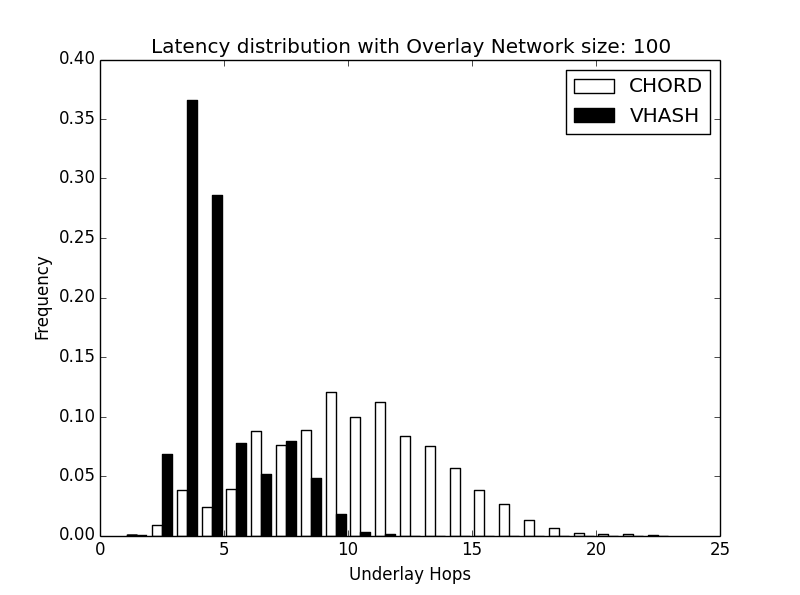
\includegraphics[width=0.5\linewidth]{figs/hist_100}
	\caption{Frequency of path lengths on Chord and VHash in a 100 node overlay.}	
	\label{fig:hist100}
\end{subfigure}

\begin{subfigure}{\columnwidth}
	\centering
	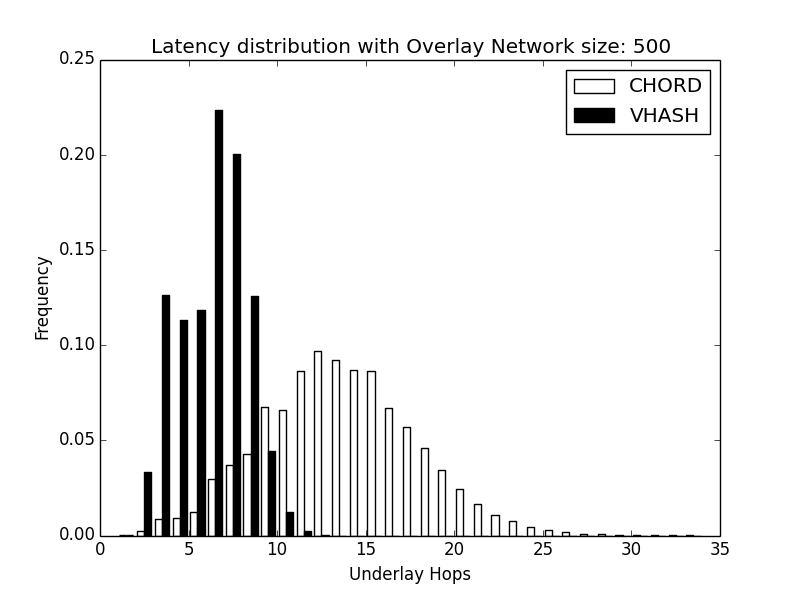
\includegraphics[width=0.5\linewidth]{figs/hist_500}
	\caption{Frequency of path lengths on Chord and VHash in a 500 node overlay.}
	\label{fig:hist500}
\end{subfigure}

\begin{subfigure}{\columnwidth}
	\centering
	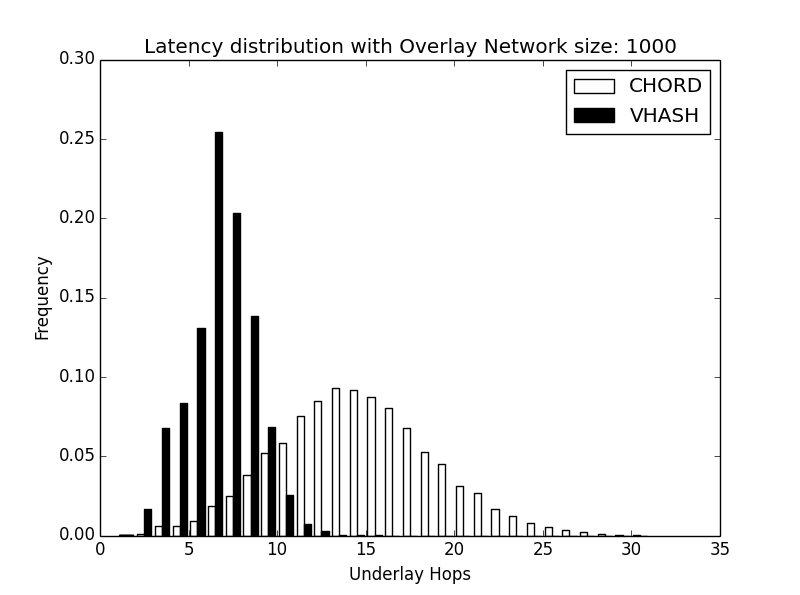
\includegraphics[width=0.5\linewidth]{figs/hist_1000}
	\caption{Frequency of path lengths on Chord and VHash in a 1000 node overlay.}
	\label{fig:hist1000}
\end{subfigure}

\caption{Figures \ref{fig:hist100}, \ref{fig:hist500}, and \ref{fig:hist1000} show the difference in the performance of Chord and VHash for 10,000 routing samples on a 10,000 node underlay network for differently sized overlays. 
The Y axis shows the observed frequencies and the X axis shows the number of hops traversed on the underlay network.
VHash consistently requires fewer hops for routing than Chord.}
\end{figure}




Figures \ref{fig:hist100}, \ref{fig:hist500}, and \ref{fig:hist1000} show the distribution of path lengths measured in underlay hops in both Chord and VHash.   
In all three network sizes, VHash dramatically outperformed Chord and significantly reduced the underlay path lengths.  
Besides having a much lower average path length, the variance was also considerably lower.

For comparison, we also sampled the lookup length measured in overlay hops for a 1000 sized Chord and VHash network.  As seen in Figure \ref{fig:histover}, the paths in VHash's overlay were significantly shorter than those in Chord. 
In comparing the overlay and underlay hops, we find that for each overlay hop in Chord, the lookup must travel 2.719 underlay hops on average; in VHash, lookups must travel 2.291 underlay hops on average for every overlay hop traversed. 
Recall that this work is based on scale free networks, where latency improvements are difficult.
An improvement of 0.4 hops over a diameter of 3 hops is significant.
VHash has on average less overlay hops per lookup than Chord, and for each of these overlay hops we consistently traverse more efficiently across the underlay network.
\begin{figure}[h]
	\centering
	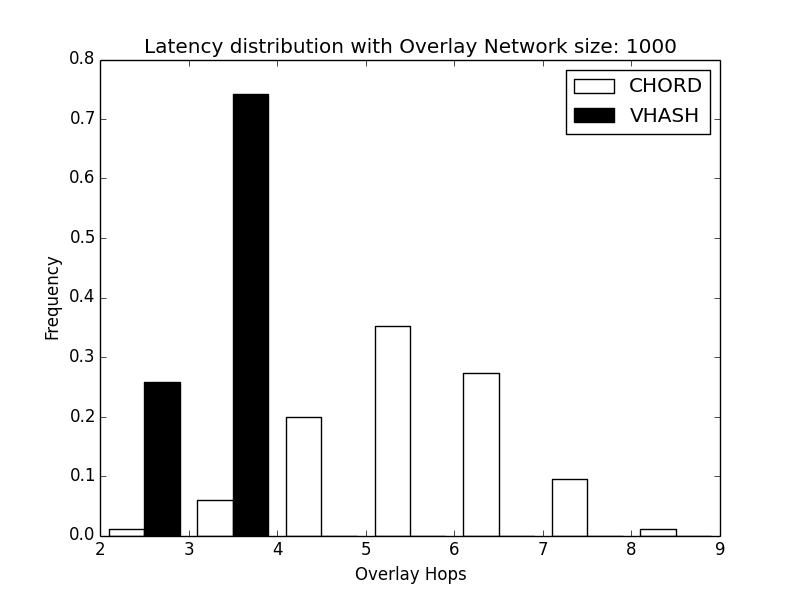
\includegraphics[width=\linewidth]{figs/hist_overlay_4d}
	\caption{Comparison of Chord and VHash in terms of overlay hops.  Each overlay has 1000 nodes.  The Y axis denotes the observed frequencies of overlay hops and the X axis corresponds to the path lengths in overlay hops.}
	\label{fig:histover}
\end{figure}




\subsection{Remarks}

Voronoi tessellations have a wide potential for applications in ad-hoc networks, massively multiplayer games, P2P, and distributed networks. 
However, centralized algorithms for Voronoi tessellation and Delaunay triangulation are not applicable to decentralized systems.
In addition, solving Voronoi tessellations in more than 2 dimensions is computationally expensive.

We created a distributed heuristic for Voronoi tessellations in an arbitrary number of dimensions.
Our heuristic is fast and scalable, with a expected memory cost of $(3d+1)^{2}+3d+1$ and expected maximum runtime of O$(\frac{\log^{2} N}{\log^{2} \log N} )$.

We ran two sets of experiments to demonstrate DGVH's effectiveness.
Our first set of experiments demonstrated that our heuristic is reasonably accurate  and our second set demonstrates that reasonably accurate is sufficient to build a P2P network which can route accurately.


Our next step is to create a formal protocol and implementation for a Voronoi tessellation-based distributed hash table using DGVH.  
We can use this DHT to choose certain metrics we want to measure, such as latency, or trust, and embed that information as part of a node's identity.
By creating an appropriate distance measurement, we can route along some path that minimizes or maximizes the desired metric.
Rather than create an overlay that minimizes hops, we can have our overlay minimize latency, which is the actual goal of most routing algorithms.

%\subsection*{Peerlist and Topology}
%Like CAN \cite{can}, VHash tracks only neighbors for it's peers.
%We enforce a lower limit on the size of the peerlist to avoid nodes being 


%\subsection*{Joining}


%\subsection*{Fault Tolerance}




\section{DHT Distributed Computing}
%TODO: Intro
Distributed computing is a current trend and is the future trend.
We see this in the development of cloud computing \cite{p2p-cloud}, volunteer computing frameworks like BOINC \cite{anderson2004boinc} and Folding@Home \cite{larson2002folding},and MapReduce  \cite{mapreduce}.
Google's MapReduce  in particular has rapidly become an integral part in the world of data processing.  
A user can use MapReduce to take a large problem, split it into small, equivalent tasks and send those tasks to other processors for computation.  
The results are sent back to the user and combined into one answer. 

Popular platforms for MapReduce, such as Hadoop \cite{hadoop}  \cite{shvachko2010hadoop}, are explicitly designed to be used in large datacenters \cite{hadoopAssumptions} and the majority of research has been focused there.  
However, as we have previously mentioned, there are notable issues with a centralized design.

First and foremost is the issue of fault-tolerance.
Centralized designs have a single point of failure \cite{shvachko2010hadoop}.
So long as all computing resources located in one geographical area or rely on a particular node, a power outage or catastrophic event could interrupt computations or otherwise disrupt the platform \cite{babaoglu2014people}.

A centralized design assumes that the network is relatively unchanging and may not have mechanisms to handle node failure during execution or, conversely, cannot speed up the execution of a job by adding additional workers on the fly.  
Many environments also anticipate a certain degree in homogeneity in the system.
Finally deploying these systems and developing programs for them has an extremely steep learning curve.

There is no reason that these assumptions need to be the case for MapReduce, or for many distributed computing frameworks in general.
Moving away from the data center context opens up more possibilities for distributed computing, such as P2P clouds \cite{p2p-cloud}.
However, without a centralized framework, the network needs some kind of protocol to organize the various components in the network.
As part of our research, we developed a highly robust and distributed MapReduce framework based on Chord, called ChordReduce \cite{chordreduce}.

There a number of reasons to used a DHT as the protocol for a distributed computing platform.
First, nodes ID and their location in the network are strongly bound to what data they are responsible for, such that any node can lookup which node is responsible a particular piece of data.
This obviates the need for a centralized organizer to maintain this bit of metadata or assign backups for data, as nodes can do this autonomously.
DHTs assume that network is heterogeneous, rather than homogeneous.
They have been used for over a decade for P2P file-sharing applications for these reasons.


%\subsubsection{P2P cloud}
%http://www.cs.unibo.it:443/pub/TR/UBLCS/2011/2011-10.pdf

%Clouds and Volunteer Computing platforms are different.
%Clouds@home
%Nanodatacenter

\subsection{ChordReduce}

ChordReduce is designed as a more abstract framework for MapReduce, able to run on any arbitrary distributed configuration.
ChordReduce leverages the features of distributed hash tables to handle distributed file storage, fault tolerance, and lookup.  
We designed ChordReduce to ensure that no single node is a point of failure and that there is no need for any node to coordinate the efforts of other nodes during processing.



\subsubsection{File System}
Our central design philosophy was to leverage as many features of the underlying DHT as possible.  
For example, we don't need to create a new distributed file system as we can just use the DHT to hash file identifiers and use the DHT to store the file at the node responsible for that key.

If the file is large, we can instead use Dabek et al.'s Cooperative File System or CFS \cite{CFS}.
In CFS, files are split into approximately equally sized blocks.  
Each block is treated as an individual file and is assigned a key equal to the hash of it's contents.  
The block is then stored at the node responsible for that key. 
The node which would normally be responsible for the whole file instead stores a \textit{keyfile}.  
The keyfile is an ordered list of the keys corresponding to the files' block and is created as the blocks are assigned their respective keys.  
When the user wants to retrieve a file, they first obtain the keyfile and then request each block specified in the keyfile.


\subsubsection{Computation}
ChordReduce treats each task or target computation as an object of data.
This means we can distribute them in the same manner as files and rely on the protocol to route them and provide robustness.


In ChordReduce, each node takes on responsibilities of both a worker node and master node, in the same way that a node in a P2P file-sharing service acts as both a client and a server.  
A user starts a job contacts a node at a specified hash address and provides it with the tasks.  
This address can be chosen arbitrarily or be a known node in the ring. 
We call this node the \textit{stager} for this particular job.  

The job of the stager divide the work into \emph{data atoms}, the smallest units of work. 
This might represent block of text, the result of a summation for a particular intermediate value, or a subset of items to be sorted. 
The specifics of how to divide the work are defined by the user in a \emph{stage} function.  
The data atoms also contain user created Map and Reduce functions.

If the user wants to perform a MapReduce job on a particular file on the network, the stager locates the keyfile for the data and creates a data atom for each block in the file.  
Each data atom is then sent to the node responsible for their corresponding block.  
When the data atom reaches it's destination node, that node retrieves the necessary data and applies the Map function.  
The results are stored in a new data atom,  which are then sent back to the stager's hash address (or some other user defined address).  
This will take $\log_{2} n$ hops traveling over Chord's fingers.  
At each hop, the node waits a predetermined minimal amount of time to accumulate additional results (In our experiments, this was 100 milliseconds).  
Nodes that receive at least two results merge them using the Reduce function.  
The results are continually merged until only one remains at the hash address of the stager. 


Some MapReduce jobs do not rely on a file stored on the network, such as a Monte-Carlo approximation
In this case, the created data atoms are then each given a random hash and sent to the node responsible for that hash address, guaranteeing they are evenly distributed throughout the network. 
From there, the execution is identical to the above scenario.


%Once the data atoms are sent out, the stager's job is done and it behaves like any other node in the network. The staging period is the only time ChordReduce is vulnerable to churn, and only if the stager leaves the ring in the middle of sending out data atoms.  The user would get some results back, but only for the data the stager managed to send out.

Once all the Reduce tasks are finished, the user retrieves his results from the node at the stager's address.  
This may not be the stager himself, as the stager may no longer be in the network.  
The stager does not need to collect the results himself, since the work is sent to the stager's hash address, rather than the stager itself.  
Thus, the stager could quit the network after staging, and both the user and the network would be unaffected by the change. % Here, we are leverging two features. First, we use the automatic assignment of responsibility to automatically route the data to the sucessor.  %Second, the same process Chord uses to backup files is used to backup the intermediate data. 

Similar precautions are taken for nodes working on Map and Reduce tasks.  
Those tasks are backed up by a node's successor, who will run the task if the node leaves before finishing its work (e.g. the successor loses his predecessor).   
The task is given a timeout by the node.  
If the backup node detects that the responsible node has failed, he starts the work and backs up again to \emph{his} successor.  
Otherwise, the data is tossed once the timeout expires.
This is done to prevent a job being submitted twice.

An advantage of our system is the ease of development and deployment.  
The developer does not need to worry about distributing work evenly, nor does he have to worry about any node in the network going down. 
The stager does not need to keep track of the status of the network.  
The underlying Chord ring handles that automatically.  
If the user finds they need additional processing power during runtime, they can boot up additional nodes, which would automatically be assigned work based on their hash value.   
If a node goes down while performing an operation, his successor takes over for him.  
This makes the system extremely robust during runtime.


\subsubsection{Robustness}
Since the system is distributed, we need to assume that any member of the network can go down at any time.
When a node fails or leaves Chord, the failed node's successor will become responsible for all of the failed nodes keys. 
Likewise, each node in the ChordReduce network relies on their successor to act as a backup.

To prevent data from becoming irretrievable, each node periodically sends backups to its successor.  
In order to prevent a cascade of backups of backups, the node sends data that it is currently responsible for.  

This changes as nodes enter and leave the network.  
If a node's successor leaves, the node sends a backup to his new successor.  
If the node fails, the successor is able to take his place almost immediately.  
This scheme is used to not only backup files, but the computational tasks as well.

This procedure prevents any single node failure or sequences of failures from harming the network. 
Only the failure of multiple neighboring nodes poses a threat to the network's integrity.  

Node's ID in the network does not map to a geographical locations.
Any failure that affects multiple nodes simultaneously would be spread uniformly throughout the network.
This means if successive nodes to fail simultaneously, they do so independently.

Let each node has failure rate $r < 1$ and that the each node backs up their data with $s$ successive nodes downstream. 
If one of these nodes fail, the next successive node takes its place and the next upstream node becomes another backup. 
This ensures there will always be $s$ backups. 
The integrity of the ring would only be jeopardized if $s+1$ successive nodes failed simultaneously.
The chances of this would be $r^s+1$, as each failure would be independent.


A final consequence of this is load-balancing during runtime.  
When a joining node $n$ find his successor, $n$ asks if the successor is holding any data $n$ should be responsible for.  
The successor looks at all the data $n$ is responsible for and sends it to $n$.  
The successor maintains this data as a backup for $n$.  
Because Map tasks are backed up in the same manner as data, a node can take the data and corresponding tasks he's responsible for and begin performing Map tasks immediately.



\subsection{Heterogeneity Calculation}

One of the advantages to using homogeneous hardware is that each machine, each core, each node is the same.
To evenly distribute the workload, you just have to give each machine the same amount of work.

This is more difficult in a heterogeneous system.
Each machine can shoulder a different amount of work.
How do we distribute work evenly across a heterogeneous system?

We can solve this by adjusting the amount of nodes representing each machine in the network.
Machines that can handle a larger load create more nodes in the network.
Besides solving the heterogeneous load-balancing problem, increasing the number of nodes in the system increases the overall load-balancing of the system.


The question we must answer is ``how?''
We need to create some unit of measurement for a distributed computing system and research if any other researchers have asked this problem.
Furthermore, this measurement might need to be relative to other nodes in the network, since the only basis for comparison are the scores of the peers.

Finally, this process needs to be handled autonomously by each node, which is the other primary focus of my proposal.
\section{Autonomous Load Balancing}
\label{sec:auto-load-bal}


During our experiments testing the capabilities of ChordReduce, we experienced a significant and completely unexpected anomaly while testing churn.
One of the things previous research \cite{marozzo2012p2p}  \cite{leemap} in the same area we felt we needed to explore better was how a completely decentralized computation could handle churn.
Now, despite our initial prototype being buggy and was only able to handle smallish networks, we were fairly certain of it's ability to handle churn.

Marozzo et al.\ \cite{marozzo2012p2p} tested their network using churn rates of 0.025\%, 0.05\%, 0.1\%, 0.2\%, and 0.4\% per minute.
The churn rate of $cr << 1$ per minute means that each minute on average, $cr \cdot n$ nodes leave the network and $cr \cdot n$  new nodes join the network.\footnote{It is standard practice to assume the joining rate and leaving rate are equal.}
This could effectively be thought of as each node flipping a weighted coin every minute.
When the coin lands on tails, the node leaves.
A similar process happens for nodes wanting to join the network.

We wanted the robustness of our system to be beyond reproach, so we tested at rates from 0.0025\% to 0.8\% \textbf{\textit{per second}}, 120 times the fastest rate used to test P2P-MapReduce.
This is an absurdly fast and unrealistic speed, the only purpose of which was to cement the robustness of the system.
Since we were testing ChordReduce on Amazon's EC2 and paying per instance per hour, we didn't use any more nodes than necessary.
Rather than having a pool of nodes waiting to join the network, we conserved our funds by having leaving nodes immediately rejoin the network under a new IP/port combo.
The meant our churn operation was essentially a simultaneous leave and join.


What we found was that jobs on ChordReduce finished twice as fast under the unrealistic levels churn (0.8\% per second) than no churn.
This completely mystified us. 
Churn is a disruptive force; how can it be aiding the network?

\subsection{Hypothesis}
We hypothesize this was due to the number of data pieces (larger) vs the number of workers (smaller).
There were more workers than there were pieces of data, so some workers ended up with more data than others in the initial distributio.
This means that there was some imbalance in the way data was distributed among nodes.
This was \textit{further} exacerbated by small number of workers distributed over a large hash space, leading some nodes to have larger swaths of responsibility than others.

Given this setup, without any churn, the operation would be:
Workers get triggered, they start working, and the ones with little work finish their work quickly, and the network waits for the node with a bunch of work.

Its important to note here that the work in ChordReduce was performed atomically, a piece at a time.
When a node was working on a piece, it informed it's successor, then informed them when it finished.
These pieces of work were also small, possibly too small.

As mentioned previously, under our induced experimental churn, we had the nodes randomly fail and immediately join under a new IP/port combination, which yields a new hash.
The failure rates were orders of magnitude higher than what would be expected in a ``real'' (nonexperimental) environment.
The following possibilities could occur:
\begin{itemize}
	\item A node without any active jobs leaves.
	It dies and and comes back with a new port chosen.
	This new ID has a higher chance of landing in a larger region of responsibility (since larger regions are larger and new joining nodes have a greater chance of hashing to that location).
	In other words, it has a (relatively) higher chance of moving into an space where it becomes acquires responsibility for enqueued jobs.
	The outcomes of this are:
	\begin{itemize}
		\item The node rejoins in a region are doesn't acquire any new jobs.
		This has no impact on the network (Case I).
		\item The node rejoins in a region that has a jobs waiting to be done.
		It acquires some of these jobs.
		This speeds up performance (Case II).
	\end{itemize}
	\item A node with active jobs dies.
	It rejoins in a new space.
	The jobs were small, so not too much time is lost on the active job, and the enqueued jobs are backed up and the successor knows to complete them.
	However, the node can rejoin in a more job-heavy region and acquire new jobs.
	The outcomes of this are:
	\begin{itemize}
		\item A minor negative impact on runtime and load balancing (since the successor has more jobs to deal with) (Case III).
		\item A possible counterbalance in load balancing by acquiring new jobs off a busy node (Case ``It probably evens out'').
	\end{itemize}
\end{itemize}

The longer the nodes work on the jobs, the more nodes finish and have no jobs.
This means as time increases, so do the occurrences of Case I and II.


This leads us to two hypotheses:
\begin{itemize}
	\item Deleting nodes motivates other nodes to work harder to avoid deletion (a ``beatings will continue until morale improves'' situation).
	\item Our high rate of churn was dynamically load-balancing the network.
	It appears even the smallest effort of trying to dynamically load balance, such as rebooting random nodes to new locations, has benefits for runtime.
	Our method is a horrible approximation of dynamic load-balancing, and it still shows improvement.
\end{itemize}

The first hypothesis is mentally pleasing to anyone who has tried to create a distributed system, but lacks rigor.
We still have to verify the existence of this phenomena in an independent experiment, and establishing that it does another goal of my dissertation.


Once we have established that it does exist, we need a better load-balancing strategy than randomly inducing.
We want nodes to have a precomputed list of locations in which they can insert nodes to perform load-balancing on an ad-hoc basis during runtime.
This precomputed list ties directly into the security research on DHTs we have done \cite{sybil-analysis}.


%The questions and goals here are straightforward:
%\begin{itemize}
%	\item Further establish the phenomena exists.
%	\item We stumbled across this phenomena with a brute force method and still got promising results.  
%	Can we create a more accurate and mean
%	\item Can this phenomena be stochastically modeled or otherwise predicted via theoretical analysis?
%	\item In what contexts can this be used for DHTs?  Distributed computing?  Replication for file sharing?

%\end{itemize}






\subsection{Sybil Attacks and Injection}
We discovered injecting replicas is easy and simple in P2P networks, we use a Sybil attack.
This was the focus of my Data Security project
I hypothesize we can Sybil attacks for improving load balancing on demand.


One of the key properties of structured peer-to-peer (P2P) systems is the lack of a centralized coordinator or authority.
P2P systems remove the vulnerability of a single point of failure and the susceptibility to a denial of service attack \cite{sybil}, but in doing so, open themselves up to new attacks.

Completely decentralized P2P systems are vulnerable to \textit{Eclipse attacks}, whereby an attacker completely occludes healthy nodes from one another.
This prevents them from communicating without being intercepted by the adversary.
Once an Eclipse attack has taken place, the adversary can launch a variety of crippling attacks, such as incorrectly routing messages or returning malicious data \cite{srivatsa2004vulnerabilities}.



One way to accomplish this attack is to perform a \emph{Sybil attack} \cite{sybil}.
In a Sybil attack, the attacker masquerades as multiple nodes, effectively over-representing the attacker's presence in the network to maximize the number of links that can be established with healthy nodes.
If enough malicious nodes are injected into the system, the majority of the nodes will be occluded from one another, successfully performing an Eclipse attack.

This vulnerability is well known \cite{dhtsec}. 
Extensive research has been done assessing the damage an attacker can do after establishing themselves \cite{srivatsa2004vulnerabilities}.
%Especially when a hash value to assign neighbors
Little focus has been done on examining how the attacker can establish himself in the first place and precisely how easily the Sybil attack can be accomplished.

We focused on looking at the computational and memory costs of creating as many replicas as possible.
The computation costs turn out to be fairly trivial and can be precomputed based on how IDs are assigned, a process I call \textit{mashing}.
If a node obtains their ID via an IP/Port combination, and we limit an attacker to using only ephemeral IP addresses (16383 total), the per node cost of mashing is quite low.
Per node, it takes 48 milliseconds to mash 16383 IP/Port combinations and only 352 kilobytes to store this information after precomputing it.


An attacker would do this for each of his nodes, then join the network and insert as many Sybils as possible.
I calculated that it would take only 1221 IP addresses to compromise 50\% of the links in a 20,000,000 node network.

An altruistic member of the network could only inject replicas where they are needed.
Given that we want nodes to insert virtual nodes, why not let nodes choose keys from the entire keyspace?
First, this is bad practice which makes a Sybil attacks trivially easy to perform.
Second, one of the primary benefits of using consistent hashing is that it allows a selection of contiguous keys to map to a uniform distribution.
Most importantly for us, this distribution can be precomputed and reproduced as needed. 
%Finally, putting constraints on what is used to generate IDs makes it more

%TODO: godfrey2005heterogeneity
\chapter{Proposed Work}

\section{Distributed DHT Computing}




Our goal is to further develop ChordReduce and release a complete verion: a DHT based platform for solving embarrassingly parallel problems using DHTs.
The steps involved in this are listed below.

\begin{itemize}
	\item We must create a highly configurable and easy to use DHT framework based off the DHT abstractions we have discovered.
	\begin{itemize}
		\item This will be done in Python3 jointly with Brendan.
		\item We will be using test driven design.
		\item The goal of this step is \textbf{not} to create a DHT, but to create an easily extensible abstract framework anyone to make DHTs.
		\item The abstraction comes from implementing the relationship we found between DHT spheres of responsibility and Voronoi tessellations
	\end{itemize}
	\item We will use the above framework to implement a few of the more popular DHTs.
	\begin{itemize}
		\item This will serve as both examples for home to implement our framework as well and the building blocks for the next step.
	\end{itemize}
	\item Implement MapReduce on these DHTs and compare their performances.
	\item Create a  processor scoring mechanism for creating virtual nodes.
	\begin{itemize}
		\item This score is a relative score, since the amount of work a node can carry is determined by the amount other nodes can carry.
		\item The score is based off of processor speed (maybe using Bogomips as the default for a while).
		\item This is compared to the scores of neighboring nodes  of all the node's replicas and should give a gauge of the node's relative processing power.
		\item This ties in directly to the autonomous load balancing.
	\end{itemize}
	\begin{itemize}
		\item The emphasis is our framework is optimized for robustness over everything else.
	\end{itemize}
	
\end{itemize}



\section{Autonomous load balancing}




%
\chapter{Previous Writing to incorporate above}





\begin{itemize}
	\item Build off of pond, make a \textit{completely} decentralized means of network programing (chordReduce)
	\item Create a method of automatic load balancing via
	\begin{itemize}
		\item inducing churn (Me: ChordReduce)
		\item injecting nodes (Me: Sybil Analysis)
		\item Replica creation (not me: IRM)
	\end{itemize}
	\item Embedding metrics into the DHT (VHash)
    \begin{itemize}
        \item Geographic location (CAN)
        \item latency 
    \end{itemize}
\end{itemize}



\section{What I need to cover}

\begin{itemize}
	\item What is my problem
	\item Why is it interesting
\end{itemize}


\section{things I have discovered and want to further explore}


\subsection{ChordReduce}
I found that churn can help out a network in ChordReduce.
It works like this-
In ChordReduce, we hypothesize this was due to the number of data pieces (larger) vs the number of workers (smaller).
There were more workers than there were pieces of data, so some workers ended up with more data than others in the initial configuration.
This means that there was some imbalance in the way data was distributed among nodes.
This was \textit{further} exacerbated by small number of workers being assigned locations with a hash function.
This leads to some nodes having larger swaths of responsibility than others.

Given this setup, without any churn, the operation would be:
Workers get triggered, they start working, and the ones with little work finish their work quickly, and the network waits for the node with a bunch of work.

It's important to note here that the work in ChordReduce was performed atomically, a piece at a time.
When a node was working on a piece, it informed it's successor, then informed them when it finished.
These pieces of work were also small, possibly too small.

Under our induced churn, we had the nodes randomly fail and  immediately join under a new ip.
The failure rates were orders of magnitude higher than what would be expected in a ``real'' (nonexperimental) environment.
The following possibilities could occur:
\begin{itemize}
	\item An node without any active jobs leaves.
	It dies and and comes back with a new port chosen.
	This new ID has a higher chance of landing in a larger region of responsibility.
	In other words, it has a (relatively) higher chance of moving into an space where it becomes acquires responsibilty for enqueued jobs.
	The outcomes of this are:
	\begin{itemize}
		\item The node rejoins in a region are doesn't acquire any new jobs.
		This has no impact on the network (Case I).
		\item The node rejoins in a region that has a jobs waiting to be done.
		It acquires some of these jobs.
		This speeds up performance (Case II).
	\end{itemize}
	\item A node with active jobs dies.
	It rejoins in a new space.
	The jobs were small, so not too much time is lost on the active job, and the enqueued jobs are backed up and the successor knows to complete them.
	However, the node can rejoin in a more job-heavy region and acquire new jobs.
	The outcomes of this are:
	\begin{itemize}
		\item A minor negative impact on runtime and load balancing (since the successor has more jobs to deal with) (Case III).
		\item A possible counterbalance in load balancing by acquiring new jobs off a busy node (Case Doesn't matter).
	\end{itemize}
\end{itemize}

Now here's the trick.
The longer the nodes work on the jobs, the more nodes finish and have no jobs.
This means as time increases, so do the occurrences that Case I and II occur, with a bit more weight on Case II.


What have we learned:
\begin{itemize}
	\item Shooting nodes as a example to motivate other nodes works or
	\item Even the smallest effort of trying to dynamically load  balance, such as rebooting random nodes to new locations, has benefits for runtime.
	Our method is a horrible approximation of dynamic load-balancing, and it still shows improvement.
\end{itemize}



We still have to verify the existence of this phenomena in an independent experiment.
Besides that, we still have the following questions:
Can I stochastically model it?
Does it work for other problems?


This ties into the next bit.
\subsection{Sybil}
We discovered injection is easy and simple in P2P networks.
I hypothesize we can Sybil attacks for improving load balancing on demand.
Perhaps we need an entirely new node type.

\subsection{VHash}
Arguablely all DHT's are Voronoi tessilations or can be mapped to.


Hops is an estimate for time, not necessarily a good one!
We can embed latency in the DHT.
We can try embedding geographic location in as well using




\subsection{Pond}
P2P can be used for decentralized volenteer computing.





\section{In WSNs}
http://users.cis.fiu.edu/~carbunar/boundary.pdf


\section{DHTs as a volunteer Platform}
Rather than rely on a centralized administrative source,


Decentralized resource discovery.
The system is organized using a P2P system built on Brunet \cite{brunet}.





\subsection{PonD}

Middleware platforms like BOINC \cite{anderson2004boinc} HTCondor\footnote{Formerly Condor; the name was changed after a copyright dispute.} \cite{thain2005distributed} provide a way to push distributed computing tasks to idle CPUs.
These platforms effectively let users donate their unused processing power to some scientific collaberative effort.

While the work is distributed, the organizational backbone  is centralized.
Scalability is the primary issue here.


On-demand computing-as-a-resource is a thing and it needs to be scalable and fault tolerant.
P2P paradigms do that.

PonD \cite{lee2012pond} does decentralized resource discovery and centralized job management/centralized scheduler.
``Decouples resource discovery from job execution/monitoring.''
Scheduling time is $ O(\log N) $, for $N$ resouces in the pool.

\subsubsection{Improvements}
Why not decentralized or partially decentralized job management?


\section{Why DHTs for distributed computing?}

\cite{malkhi2001viceroy} -  Between congestion, cost of join/leaves, and lookup time there are tradeoffs.  
Optimizing for two can be done but has bad cost.
For example, a balanced binary tree has congestion at root.


\section{MapReduce}

%copied from CHRONUS
Google's MapReduce \cite{mapreduce} paradigm has rapidly become an integral part in the world of data processing and is capable of efficiently executing numerous Big Data programming and data-reduction tasks.  
By using MapReduce, a user can take a large problem, split it into small, equivalent tasks and send those tasks to other processors for computation.  
The results are sent back to the user and combined into one answer.  
MapReduce has proven to be an extremely powerful and versatile tool, providing the framework for using distributed computing to solve a wide variety of problems, such as distributed sorting and creating an inverted index \cite{mapreduce}. 

At it's core, MapReduce \cite{mapreduce} is a system for process key/value pairs, a that statement that equally describes DHTs.
However, MapReduce operates over a different set of assumptions \cite{hadoopAssumptions} than DHTs.
MapReduce platforms are highly centralized and tend to have single points of failure\cite{shvachko2010hadoop} as a result.   
A centralized design assumes that the network is relatively unchanging and does not usually have mechanisms to handle node failure during execution or, conversely, cannot speed up the execution of a job by adding additional workers on the fly.
Finally deploying these systems and developing programs for them has an extremely steep learning curve.

If we make MapReduce operate under the same assumptions as a DHT, we have effectively further abstracted the MapReduce paradigm and created a system that can operate both in a traditional large datacenter or as part of a P2P network.
The system would be highly resistant to failures at any point, scalable, and automatically load-balance. 
The administrator can add any number of heterogeneous nodes to the system to get it operate.

\subsection{Current MapReduce DHT/P2P combos}
There have been a few implementations combining MapReduce with a P2P framework, in varying capacities.  
I will present two here, as well as my own implementation, ChordReduce.

\subsubsection{P2P-MapReduce}
Marozzo et al. \cite{marozzo2012p2p} investigated the issue of fault tolerance in centralized MapReduce architectures such as Hadoop.  
They focused on creating a new P2P based MapReduce architecture built on JXTA called P2P-MapReduce.  
P2P-MapReduce is designed to be more robust at handling node and job failures during execution.

Rather than use a single master node, P2P-MapReduce employs multiple master nodes, each responsible for some job.  
If one of those master nodes fails, another will be ready as a backup to take its place and manage the slave nodes assigned to that job.  
This avoids the single point of failure that Hadoop is vulnerable to. Failures of the slave nodes are handled by the master node responsible for it.

Experimental results were gathered via simulation and compared P2P-MapReduce to a centralized framework. 
Their results showed that while P2P-MapReduce generated an order of magnitude more messages than a centralized approach, the difference rapidly began to shrink at higher rates of churn.  
When looking at actual amounts of data being passed around the network, the bandwidth required by the centralized approach greatly increased as a function of churn, while the distributed approach again remained relatively static in terms of increased bandwidth usage. 
They concluded that P2P-MapReduce would, in general, use more network resources than a centralized approach. 
However, this was an acceptable cost as the P2P-MapReduce would lose less time from node and job failures \cite{marozzo2012p2p}.

\subsubsection{Parralel Processing Framework on a P2P System}
Lee et al.'s work \cite{leemap} draws attention to the fact that a P2P network can be much more than a way to distribute files and demonstrates how to accomplish different tasks using Map and Reduce functions over a P2P network.  
Rather than using Chord, Lee et al. used Symphony \cite{symphony}, another DHT protocol with a ring topology.  
To run a MapReduce job over the Symphony ring, a node is selected by the user to effectively act as the master.  
This ad-hoc master then performs a bounded broadcast over a subsection the ring.  
Each node repeats this broadcast over a subsection of that subsection, resulting in a tree with the first node at the top.  

Map tasks are disseminated evenly throughout the tree and their results are reduced on the way back up to the ad-hoc master node.  
This allows the ring to disseminate Map and Reduce tasks without the need for a coordinator responsible for distributing these tasks and keeping track of them, unlike Hadoop.  
Their experimental results showed that the latency experienced by a centralized configuration is similar to the latency experienced in a completely distributed framework.





\subsubsection{ChordReduce}
ChordReduce is designed as a more abstract framework for MapReduce, able to run on any arbitrary distributed configuration.
ChordReduce leverages the features of distributed hash tables to handle distributed file storage, fault tolerance, and lookup.  
ChordReduce  was designed to ensure that no single node is a point of failure and that there is no need for any node to coordinate the efforts of other nodes during processing.  



\subsection{Experiment Description: Comparison of MapReduce paradigm on different DHTs}
In order to test MapReduce over a DHT, I will do the following:
\begin{itemize}
	\item Implement CAN \cite{can}, Pastry \cite{pastry}, Chord \cite{chord}, Kademlia \cite{kademlia}, VHash, and ZHT \cite{li2013zht} /similar
	\begin{itemize}	
		\item This covers different geometries with different base parameters.
		\item This also necessitates the creation of an extensible DHT framework.
		\item  The DHT should be extended with more powerful search functionality (see distributed database below), and built-in policies for virtual nodes.
		
	\end{itemize}
	\item Compare results with each other and a traditional MapReduce platform, such as Hadoop.
	\item Certain DHTs may be better suited to different problem formulation
	
\end{itemize}



%\section{High End Computing}
%PonD?
%\subsection{Metadata Management}
%\subsection{Robustness}

%\subsection{Experiment Description:}

%\section{Graph Processing on a DHT} 
%Lookup Graphlab
%\subsection{Embedding}

%\subsection{Experiment Description:}
%\subsection{Distribute the work for solving a graph on a DHT}
%\subsection{Comparison to well established or state of the art methods}



%\section{Machine Learning Problems on A DHT}


%\subsubsection{Bayesian Learning}
%%\subsection{Experiment Description:}
%Take MapReduce machine learning algorithm

\section{Distributed ``Databases'' and Complex Queries}


DHTs run off the assumption that you know what you want to find.
I'm looking for node responsible for this key, becuase I need the associated value.

Complex queries and databases are used to find stuff based on attributes, and since you're asking, you don't know what (primary) keys you need.


Want to find all files that match the criteria?





Simple: Find all files with ``author = John Smith''.  Idiot solution, assign ``author = John Smith'' a hash key,  it's value is a file with all the files with the (that doesn't scale) 


Complex: Processing database queries.   Find all files with age < 20 and niceness >12

One proposed soultion is to use montonic (order-preserving) hash functions \cite{triantafillou2004towards}, but monotonic functions don't have randomness and uniformity.


Could embed as dimension with VHash!


See lee pond for their multi-tree broadcast which they got from other papers \cite{lee2012pond}



Koorde?HpyerChord
Each node has it's own subset chord ring

Query to a space, then within the space, deluge and spam the query which gives a reduce path
\subsection{Paper summaries}

P2P systems have two limitations: scaling and complex queries \cite{harren2002complex}.  
I would also say robustness.
DHTs have solved the issue of sclaing for the most part but have a significantly limitted querying capability:  only native-exact matches are supported.  

A database is to be avoided since most users will not want to manage a database.  
The authors wish to focus purely on the abstract relational algebra operations, since the objective is only query processing.

The authors proposed extending the DHT API.
The data storage layer needs a way to iterate thru the data objects it has stored.
Each object needs a unique local identifier and the data itself, as well as a way of accessing stored metadata for each object. 


A big issue is supporting the range queries, since exact matches can be solved in many different ways.
One proposed soultion is to use montonic (order-preserving) hash functions \cite{triantafillou2004towards}, but monotonic functions don't have randomness and uniformity.

Triantafillou et al.\ propose keying the ID of file off the primary key of a relation and using an order-preserving hash function for each of the other attributes.\footnote{This technique was designed only for \texttt{ints}}
For each attribute $DA_i$, the entire keyspace is partitioned into $s_i = \frac{2^{m}}{|DA_{i}|}$ and the monotonic hash function $h_i$ for $DA_i$ is defined as  $h_{i}(a_{i})=\lceil (a_{i} - \min(DA_i)) \times s_i \rceil$ for each individual attribute $a_i$  (may have botched terminology).


When a tuple with key $t$ is \texttt{put} on the network, it's stored at \texttt{successor(t)}.  It is then replicated at each peer responsible for each attribute, which is found using the order-preserving hash functions.


\subsubsection*{PHT}
%Abstract level summary.  What can it do, what can't it do.


\section{Semiautomagic Load Balancing}
What: Automagic load balancing.  One of two possiblilities:  inject new node into region or create new virtual node in region. 
Requires Where, when, and how/which

\begin{itemize}
    \item Where: Can be answered with Sybil selection.
    \item When:  Can be answered with IRM for hot spots.  Can be answered with neighbor monitoring
    \item How:  The remaining peace
    \item Symphony demonstrates how to estimate $n$
\end{itemize}

2/28: joiner asks parent holds the most, who asks his log n nodes who holds the most


Need equation for optimal number of replicas in the network.

\section{Resources}
\subsection{Planetlab}
\subsection{Local Cluster}


\bibliography{notes,dht,mapreduce,voronoi,dns,botnets}
\bibliographystyle{plain}
\end{document}





